\documentclass[10pt]{report}
\usepackage[centertags]{amsmath}
\usepackage{amsfonts}
\usepackage{amssymb}
\usepackage{amsthm}
\usepackage{newlfont}
\usepackage{graphicx}
%\usepackage[super,sort&compress]{natbib}
%\usepackage[sort&compress]{natbib}
%\usepackage[numbers]{natbib}
\usepackage[authoryear,square]{natbib}

\hfuzz2pt
\newlength{\defbaselineskip}
\setlength{\defbaselineskip}{\baselineskip}
\newcommand{\setlinespacing}[1]%
           {\setlength{\baselineskip}{#1 \defbaselineskip}}
\newcommand{\doublespacing}{\setlength{\baselineskip}%
                           {2.0 \defbaselineskip}}
\newcommand{\singlespacing}{\setlength{\baselineskip}{\defbaselineskip}}
\newcommand{\A}{{\cal A}}
\newcommand{\h}{{\cal H}}
\newcommand{\s}{{\cal S}}
\newcommand{\W}{{\cal W}}
\newcommand{\BH}{\mathbf B(\cal H)}
\newcommand{\KH}{\cal  K(\cal H)}
\newcommand{\Real}{\mathbb R}
\newcommand{\Complex}{\mathbb C}
\newcommand{\Field}{\mathbb F}
\newcommand{\RPlus}{[0,\infty)}
\newcommand{\norm}[1]{\left\Vert#1\right\Vert}
\newcommand{\essnorm}[1]{\norm{#1}_{\text{\rm\normalshape ess}}}
\newcommand{\abs}[1]{\left\vert#1\right\vert}
\newcommand{\set}[1]{\left\{#1\right\}}
\newcommand{\seq}[1]{\left<#1\right>}
\newcommand{\eps}{\varepsilon}
\newcommand{\To}{\longrightarrow}
\newcommand{\RE}{\operatorname{Re}}
\newcommand{\IM}{\operatorname{Im}}
\newcommand{\Poly}{{\cal{P}}(E)}
\newcommand{\EssD}{{\cal{D}}}
\theoremstyle{plain}
\newtheorem{thm}{Theorem}[section]
\newtheorem{cor}[thm]{Corollary}
\newtheorem{lem}[thm]{Lemma}
\newtheorem{prop}[thm]{Proposition}
\theoremstyle{definition}
\newtheorem{defn}{Definition}[section]
\theoremstyle{remark}
\newtheorem{rem}{Remark}[section]

\newcommand{\field}[1]{\mathbb{#1}}
\newcommand{\C}{\field{C}}
\newcommand{\R}{\field{R}}
\newcommand{\script}[1]{\mathcal{#1}}
\DeclareSymbolFont{AMSb}{U}{msb}{m}{n}
\DeclareMathSymbol{\dbln}{\mathalpha}{AMSb}{"4E}
\DeclareMathSymbol{\dblp}{\mathalpha}{AMSb}{"50}
\DeclareMathSymbol{\dblz}{\mathalpha}{AMSb}{"5A}
\DeclareMathSymbol{\dblr}{\mathalpha}{AMSb}{"52}
\DeclareMathSymbol{\dblt}{\mathalpha}{AMSb}{"54}
\DeclareMathSymbol{\dblq}{\mathalpha}{AMSb}{"51}
\DeclareMathSymbol{\dbln}{\mathalpha}{AMSb}{"4E}
\DeclareMathSymbol{\dblf}{\mathalpha}{AMSb}{"46}
\DeclareMathSymbol{\dblc}{\mathalpha}{AMSb}{"43}
\DeclareMathSymbol{\dbld}{\mathalpha}{AMSb}{"44}
\newcommand{\fall}{\; \forall \;}
\newcommand{\exts}{\; \exists \;}
\newcommand{\st}{\; \ni \;}
\newcommand{\mbf}[1]{\mathbf{#1}}
\newcommand{\binomial}[2]{\biggl( \begin{array}{c}  #1 \\ #2  \\ \end{array} \biggr) }
\newcommand{\fderiv}[2]{ \frac{d}{ d #1} \: #2}
\newcommand{\sderiv}[2]{ \frac{d^2}{ d^2 #1} \: #2}
\newcommand{\pfderiv}[2]{ \frac{\partial}{ \partial #1} \: #2}
\newcommand{\psderiv}[2]{ \frac{\partial^2}{ \partial^2 #1} \: #2}
\newcommand{\mat}[1]{\mathbf{#1}}

\numberwithin{equation}{section}
\renewcommand{\theequation}{\thesection.\arabic{equation}}

\title{A Field Guide for Machine Learning, Computer Vision and Numerical Linear Algebra}

\author{Bruce B. Campbell}

\begin{document}

{ \typeout{A Field Guide for Machine Learning, Computer Vision and Numerical Linear Algebra}
\include{ABS}
}

{ \typeout{Acknowledgements}
\include{ACK}
}
\def\baselinestretch{1}
\setlinespacing{1.5}

\setcounter{page}{1}
\tableofcontents

{ \typeout{Introduction}

This work addresses
\begin{quote}
{\em the application and implementation of techniques in Machine Learning, Statistical Pattern
Recognition, \& Spectral Graph Theory }
\end{quote}
to {\em problems in real world data analysis}.

\medskip

}

\setlinespacing{1.5}
\newcommand{\footn}[1]{\footnote{\hspace{0.1cm}\parbox[t]{13.25cm}{#1}}}
\section{Learning Theory and Functional Analysis}
Supervised learning in its most abstract setting requires finding a function $f(x)$ given instances ${ (x_i ,f(x_i))}$. Typical assumptions are that ${x_i}$ is an iid sample from some unknown distribution. A loss function is a random variable \[ L : Ran(f) \times Ran(f) \rightarrow \dblr^+\] defining the cost of misclassification.  The risk associated with a candidate function $f'$ is defined to be the expectation of the loss over the sample space $\Omega$, \begin{equation} R(f')=\int L( f(\omega), f'(\omega)) d\omega\end{equation}.  Statistical learning theory is concerned with assessing the approximations to $f$ given by minimizing the empirical loss associated with a sample ${ (x_i ,f(x_i))}$.

The notion of a loss function goes back to the roots of modern probability theory and economics. The St. Petersburg paradox is an example of a random variable $S : \dbln \rightarrow \dblr^=$ with infinite expectation limited utility. Let $W(k)$ be the winnings after k plays of from a game with outcome $S$ that pays $2^{i-1}$ with probability $p_i=1/2^i$. $\lim_{k\To\infty} W(k)/k =E(S)=\sum\limits_{i=1}^{\infty} p_i 2^{i-1}= \infty$ The implication for a decision theory based only expected value is that a rational player would pay an infinite amount of money to play this game. Bernoulli introduced the notion of expected utility which takes into account the fact that a payout of $2^i$ may not have twice the utility of a payout of $2^{i+1}$ when $i$ gets large.  The utility $U$ is a random variable on the sample space representing preferences of an agent.  Loss represents the aversion of an agent to the outcomes of the sample space, \[L(\omega)+U(\omega) = \alpha \fall \omega \in \Omega\] where $\alpha$ is constant.  Expected loss $R(f')$ is the risk associated with choosing the approximation $f'$. Restricting the class of functions to consider when minimizing the risk for a candidate approximation to $f$ is a key aspect of classifier design.

Gaussian processes provide a class of models and learning algorithms for real world problems that have a long history and are well characterized. Learning algorithms are cast as minimization problems $min_\mathcal(H) R() $ in a Hilbert space $ \mathcal{H}$ with a dot product that encapsulates a model and sample data.  Bayesian methods are often employed for estimation and inference with Gaussian processes. They allow an intuitive approach to incorporating prior knowledge in classification problems and the ability to obtain confidence intervals for predictions.  Many common regression and classification algorithms can be cast as minimization problems in a Reproducing Kernel Hilbert Space (RKHS).


\section{Learning With Kernels}


\cite{KLBurges98atutorial}, \cite{KLKeerthi99improvementsto}, \cite{KLProgramminglearningthe},
\cite{KLScholkopf00newsupport}, \cite{KLScholkopf00statisticallearning}, \cite{KLShevade99improvementsto},
\cite{KLTsang03distancemetric}, \cite{KLWeston00featureselection}, \cite{KLSchultz03learninga}

Kernel learning is a paradigm for classification and regression where prior belief is expressed in the construction of a similarity matrix of distanced between points in a feature space $\Omega$ by embedding via a non linear map $\phi$ in a higher [often infinite] dimensional Hilbert space using the kernel as an inner product.
\begin{center}\begin{eqnarray*}
% \nonumber to remove numbering (before each equation)
  K(x,x')= <\phi(x),\phi(x')> \\
  K \succeq 0 \\
  SPD \Rightarrow \sum\limits_{x \in \Omega}^{}  \sum\limits_{x' \in \Omega}^{} f(x) K(x,x') f(x') \geq 0 \forall f\ \in \ell^2(\Omega)
\end{eqnarray*}\end{center}
Recall that infinitely divisible probability distributions aries as the sum of $iid$ random variables.  Infinitely divisible kernels have the representation
\begin{center}\begin{eqnarray*}
K=K^{\frac{1}{n}} \ldots K^{\frac{1}{n}} \\
K= e^{\beta H} \\
e^{\beta H} = \lim\limits_{n\rightarrow \infty} (1+ \frac{\beta H}{n} )^n
\end{eqnarray*}\end{center}
We construct a mutli-resolution representation of the data with exponentiated kernels.  The sequence of kernels $K(\beta)$ represents a one parameter group associated with a diffusion on the graph of the data.  A $\beta \rightarrow  0 \infty$ the kernel moves from the identity to one that represents the clusters in the off diagonal components.  The local structure of $\Omega$ is preserved in $H$ while the global geometry of the data set is progressively revealed in $K(\beta)$ as we push the diffusion forward with the one parameter group.  We can construct exponentiated kernels over direct products of sets $\Omega_1 \bigotimes \Omega_2$ that will allow for the class conditional representation [bbcrevisit term use multiclass].  Simply set $H = H_1 \bigotimes I_{\Omega_1} +  H_2 \bigotimes I_{\Omega_2}$.
\begin{center}\begin{eqnarray*}
K(\beta) = e^{\beta H} =  e^{(\beta H_1 \bigotimes I_{\Omega_1} +  H_2 \bigotimes I_{\Omega_2})} \Rightarrow \\
\frac{d}{d \beta} K(\beta) =  H (K_1(\beta) \bigotimes K_2(\beta))
\end{eqnarray*}\end{center}

The kernels thus  constructed can be used to drive a diffusion on a graph by letting $H$ be the familiar graph Laplacian.  Furthermore, the continuum limit of infinite data can be analyzed in within the framework of a discreet stochastic process much the way the convergence of finite element solutions of PDE's takes place.


\section{Kernel Density Estimation}
To define the empirical distribution function of a sample of size $N$ - place mass $1/N$ at each member of the sample.  This forms a nonparametric estimate of the marginal density $P(X)$.  This is a singular form of kernel smoothing for density estimation.  If $\psi$ belongs to some nice class of function, and $\int\limits_{\infty}^{-\infty}\psi(x) dx = 1$, we can form a parametric estimator for the pdf of a process from a sample
population of size $N$ by calculating
\begin{equation} p(x;\theta)=\frac{1}{N \theta}
\sum\limits_{i-1}^{N} \phi( \frac{x-X_n}{\theta})
\end{equation}  If $\phi$ happens to be a density then $p(x,
\theta)$ is also a density.  Letting $\theta \rightarrow 0$ for
the right kernel, we get the empirical density of the sample
%bbcrevisit - provide kernel that makes the limit ok
population.  The mean squared error of the estimator expressed
as a bias term and a variance term is \begin{equation} Err
p(x;\theta)= E[p(x;\theta)-p(x)]^2 =  E[ p(x;\theta)-p(x)]^2 =
(E[p(x;\theta)]-p(x))^2 + Var[ p(x;\theta)]
\end{equation}


\section{Distance Functions \& The Affinity Matrix}

There are two key ingredients to forming the affinity matrix; a distance function, and a convention for which pairs to consider.  If all or too many pairs are compared, sparse methods will not be possible.  We can include $n$ nearest points, all points within $\epsilon$ of $x$, or some other criteria. For instance when working with spatial data, the diffusion can be done on a graph formed by a tessellation of the locations.  This is exactly how numerical solutions of heat diffusions are done.

BBCREVISIT - Gram Matrix \& Mercers Theorem - Make sure we connect to SVM section.

If the feature vector is a histogram, the $L^2$ distance is not meaningful, in this case use the $\chi^2$

\section{The Graph Cut}
Spectral clustering is a relaxation to an NP-hard problem of finding an optimal way to cut a graph. Here we describe some various cut criteria.  Let
\begin{eqnarray*}
X_1, \hdots , X_n \; \in \dblr^n  \\
W_ij = s(X_i,X_j)
d_i = \underset{\sum}{j} W_{i j}
|A| = card (A)
vol(A) = \underset{\sum}{i \in A} d_i
\end{eqnarray*}

BBCREISIT - Find ref, fill in defs, and possibly demo on small graphs.
\begin{defn}[Min Cut]
\begin{equation*} min cut(A,B) =\underset{\sum}{i \in A \; j \in B}  W_ij \end{equation*}
\end{defn}

\begin{defn}[Balanced Cut / Ratio Cut ]
\begin{equation*} min cut (A,B) \frac{1}{|A|} \frac{1}{|B|} \end{equation*}
\end{defn}

\begin{defn}[n Cut ]
\begin{equation*} min cut (A,B) \frac{1}{vol(A)} \frac{1}{vol(B)} \end{equation*}
\end{defn}



\section{Graph Spectra}
Graph spectral methods are some of the most successful heuristic approaches to partitioning algorithms in solving sparse linear systems, clustering and, ranking problems.  Eigenvalues of the graph Laplacian are used to transform a combinatorial optimization problem to a continuous one, typically a SDP problem.  Recent advances in SDP optimization techniques have opened new avenues of research in combinatorial optimization.  For instance, isoperimetric properties of a graph are used to find efficient communication networks, and fast convergence of Markov Chains.



\section{Matrix Factorization}
Many forms of matrix factorization can be cast as an optimization problem that involves minimization of generalized Bregman divergences\cite{BDAUnifiedViewMatrixFactorizationModels}.  Factorization algorithms such as  NNMF, Weighted SVD, Exponential Family PCA, , pLSI, Bregman co-clustering \cite{CCBanerjee04ageneralized} can be cast in this framework.  The approach uses an alternating projection algorithm for solving the optimization problem which allows for generalizations that include row, column, or relaxed cluster  constraints.  A brief description of the algorithm is given below.  The description of a generalized Bregman divergence can be found in \cite{BDGordon99approximatesolutions}.



\section{PCA and its generalization to the Exponential Family}
PCA finds linear combinations of the variables that correspond to directions of maximal variance in the data. Typically this is performed via a singular value decomposition (SVD) of the data matrix $A \in R^{n,m}$, or via an eigenvalue decomposition if A is a covariance matrix in which case $A \in R^{n,n}$. Representing the data in the directions of maximum variance allows for a dimension reduction that preserves information. Principal component directions are uncorrelated which can be useful.  PCA has the disadvantage that components are usually linear combinations of all variables. Weights in the linear combination data elements are non-zero. Sparse PCA is an attempt to find a low dimension representation of the data that explainers most of the variance.

Here we describe a generalization  of Principal component analysis (PCA) to the Exponential Family of probability distributions.  PCA is a popular dimensionality reduction technique that seeks to find a low-dimensional subspace passing close to a given set of points \begin{equation*}\{x_i\} \subset \mathbb{R}^n\end{equation*}.  The procedure is to solve the optimization problem that minimizes the sum of squared differences of the data points to the projections on a subspace spanned by the empirical variance after centering the data to have mean $0$;
\begin{equation*}
\sum\limits_{i=i}^{n} \norm{x_i - \theta_i}^2_{\ell^2}
\end{equation*}.  The choice of $\ell^2$ norm here codifies the assumption of Gaussian data.  An alternate interpretation of the algorithm is finding the  parameters ${\theta_i}$ that maximizes the log likelihood of the data which corresponds to \begin{equation*}
\sum\limits_{i=i}^{n} \norm{x_i - \theta_i}^2_{\ell^2}
\end{equation*}.  The goal of PCA is to find the the true low dimensional distribution   of the data given the assumption that data is corrupted by Gaussian noise.
Bregman divergences
  \begin{equation*}
  D_\phi(A,B)=\phi(A)-\phi(B) - \nabla \phi(B) (A-B)
\end{equation*}
offer a framework to extend PCA [and other spectral dimension reduction techniques] to the entire Exponential Family.  Here $\phi$ is a striclty convex function.  The roles of

Let  $\theta_i$ be the natural parameter for dimension $i$, with Exponential distribution $P_\theta$.  Then the conditional expectation is given by
\begin{equation*}
log P_\theta (x| \theta) = log P_0(x) + x \theta - G(\theta)  \sp : G \ni \int{ P_\theta dx} =1
\end{equation*}
We can model multivariate data where the conditional distribution can vary along the feature space.  The common feature of this PCA model and GLZ regression is the derivative of $G$ which is familiar link function and the loss function which is appropriate for $P_\theta (x | \theta)$.  The non linear relationship in the GLZ regression model data is captured by the link function $h = \frac{d}{d \theta}G(\theta)'$.  This feature is also passed on to the generalized PCA.  Instead of projecting on to a linear subspace, a Bregman divergence is used as the distortion measure.  This gives a convex optimization problem to solve which can be shown to converge.  In \cite{BDAzoury99relativeloss} a dual function  to  $\phi$ is defined by the relationship $\phi(g(\theta))+G(\theta)=h(\theta) \theta$ which is used to write the log likelihood as a Bregman divergence
\begin{equation*}
    \log P( x | \theta ) = -log P_0(x) - \phi(x) + D_\phi (x,h(\theta))
\end{equation*}.  Typically $x$ is a vector but extending to matrices is straightforward.


Sparse PCA
[CS Notes from http://ugcs.caltech.edu/~srbecker/

Classic PCA is sensitive to outliers.  Convex methods can be use to address this by attempting to factor the data $X$ as a sum of a low rank component $L$ and a sparse component $S$ by solving
\begin{equation*}
\underset{min}{S,L} \norm{L}_* + \lambda \norm{S}_{\ell_1}  : X=L+S
\end{equation*}
See http://cvxr.com/tfocs/demos/rpca/ for a demo of this in action with the popular cvx software package.


\section{Manifold Learning}
There are numerous machine learning techniques which accomplish some form of dimensionality reduction.
Manifold learning uses principal curves and manifolds to encode a natural geometric framework for nonlinear dimensionality reduction.  These methods construct low-dimensional data representation using a cost function that retains local properties.
Contrasting methods such as MDS employ proximity data via a similarity or distance matrices.  The important ISOMAP \cite{MDS_ISOMAP}algorithm extends MDS by capturing geodesic measurements of non-local pairs on the data manifold $M$ via an multi-scale approximation.  Non-local distances are approximated via a shortest path on a K nearest neighbor clustering of the data.  Effectively a ball in data space is used to represent a cluster, and a graph is then constructed to encode the non-local information.  The connectivity of the data points in the neighborhood graph are the nearest k Euclidean neighbors in the feature space.  Dijkstra's algorithm for computing shortest paths with weights is used to construct the proximity matrix from the neighborhood graph.  The top n eigenvectors encode the coordinates in the low dimensional Euclidean space.  Choosing the correct number of neighbors is an essential component to an accurate representation.
Other shortest path algorithms that may be employed to calculate the geodesic distances are listed below:
\begin{itemize}
  \item Dijkstra's algorithm finds the single-pair, single-source, and single-destination shortest path.
  \item Johnson's algorithm finds all pairs shortest paths
  \item Bellman-Ford algorithm single source problem and allows negative edge weights.
  \item Floyd-Warshall algorithm solves all pairs shortest paths.
  \item A* search algorithm solves the single pair shortest path problem.
\end{itemize}
In \cite{MDSBernstein00graphapproximations} a sampling condition is given which bounds the quality of the manifold embedding based on the quality of the neighborhood graph.


\section{Graph Laplacian}
\cite{GLPBoydconvexoptimization}, \cite{GLPChung93laplaciansof}, \cite{GLPCrescenzi96toweight},
\cite{GLPGuatterygraphembeddings}, \cite{GLPBoydconvexoptimization},
\cite{GLPChung93laplaciansof},
\cite{GLPSpectralAnalysisComplexLaplacianMatrices}, \cite{GLPKellersignedgraph}

Let $G$ be a connected simple graph with vertex set $V = {1, 2, ... , n}$ , edge set $E$ and let each edge be associated with a positive number, called the weight of the edge. The above graph is called a weighted graph. An unweighted graph is just a weighted graph with each of the edges bearing weight 1.  The weight $w(i)$ of a vertex $V_i$ is the sum of the weights of the edges incident with it. There are a number of ways in which the  Laplacian matrix $L$ is defined; the combinatorial Laplacian, the normalized Laplacian and the unsigned Laplacian.  Spectra from graph matrix representations may be obtained from the adjacency matrix $A$ and the various Laplacian discretizations.  Spectra can also be derived from the heat kernel matrix and path length distribution matrix.

The matrix representation of the graph Laplacian has a significant effect on the spectrum.  Attributes may be accounted for by by a complex number that encodes the edge attributes.  The node attributes may be encoded in the diagonal elements.   The complex graph Laplacian matrix is Hermitian, and hence it has real eigenvalues and complex eigenvectors.  Graph feature vectors can be embedded in a pattern space by PCA, MDS, and LDA( linear discriminant analysis).  Attribute graphs may be characterized by the application of symmetric polynomials to the real and complex components of the eigenvectors. \cite{GLPAnaFred} This gives rise to permutation invariants that can be used for pattern vectors.  Partitioning a graph into three pieces, with two of them large and connected, and the third a small separator set can be accomplished using the second eigenvector [the Feidler Vector] of the graph Laplacian.  In the case or sparse graphs, the first few eigenvectors can be efficiently computed using the Lanczos algorithm [see section below on ARPAC].  This graph partitioning algorithm can be extended to give a hierarchical subdivision of the graph.


\section{Distance Metrics}
A measure of similarity between data points is a vital component to clustering algorithms.  The suitability of any given measure is dependent on the generative process providing the data.


\section{Markov Chains}
Let $X \in \mathcal{M}$, $P(x,y)$ the transition probability for an irreducible Markov chain. If $P$ is reversible relative to $\pi$ then we have that $Q(x,y) = \Pi(x) P(x,y) =\Pi(y) P(y,x) \forall x,y, \in X$.  This implies that $\pi$ is the stationary distribution.  Bounding the rate of convergence to the stationary distribution is related to $L_G$ and isoperimetric problems.

Detailed balance is a property of a Markov chain where $\pi(x) P(x,y) =\pi(y) P(y,x) \Rightarrow$ reversibility.  This is stronger than the requirement of a stationary distribution.  It is the property that implies for every closed cycle of states there is no flow of probability.

There are four aspects of Markov chain stability.
\begin{enumerate}
\item $\pi$-irreducible
\item small set
\item Harris recurrence
\item Geometric Ergodicity
\end{enumerate}

For reversible Markov chains, the rate of convergence to $\Pi$ for a finite state chain is determined by the second eigenvalue of $P$.

There are two types of bounds for the rates of convergence
\begin{enumerate}
\item graph theoretic Cheeger type - see Diaconis and Stook
\item Spectral
\end{enumerate}
The rate of convergence to $\pi$ for finite state Markov chains is determined by the second eigenvalue $\lambda_2$ of $P$.

BBCREVISIT CLEAN UP LOTS
\begin{thm}[Perron Frobenius - $P \in \dblp^{n \times n}$ ]
There is a simple largest eigenvalue, and it's eigenvector is positive.

\end{thm}
The growth of $P^k$ is determined by the Perron eigenvalue.  Frobenious extended the theorem to include a class of non negative matrices.  This is achieved through the concept of reducibility.  $P$ is irreducible if
\begin{equation*}
\neg \exists \; \Lambda \st\Lambda^\dag L \Lambda =
 \left( \begin{array}{cc}
P_{11} & P_{12}  \\
0 & P_{22} \end{array} \right)
\end{equation*}
where $\Lambda$ is a projection $\Lambda^2 = \Lambda$
The irreducible matrices $L$ have a simple largest eigenvalue $\lambda_n$, now called the Perron-Frobenius eigenvalue whose right eigenvector components are all positive.  We can put this in Markov chain terminology; irreducibility is equivalent to the existence of a unique stationary distribution.

BBC Make the Markov Chain section nice.

Hammerlsy Clifford

The Hammersley–Clifford theorem gives necessary and sufficient conditions for when a positive probability distribution can be represented as a Markov Random Field. It states that a probability distribution that has a positive mass or density satisfies one of the Markov properties with respect to an undirected graph $G$ if and only if it is a Gibbs random field.  The density of the Gibbs random field can be factorized over the cliques (complete subgraphs) of $G$.


\section{Spectral Graph Theory}
Modern spectral graph theory increasingly takes insights from geometry.  Discrete analogues of isoperimetry results and heat flow on manifolds are just a few examples being put to use in modern applications.  The normalized graph Laplacian is used to aid in consistency between spectral geometry and stochastic processes.  We consider connected graphs $G = (E,V)$ in this work, in which case we can define the normalized graph Laplacian as $\mathcal{L} = T^{\frac{1}{2}} L T^{\frac{-1}{2}} = I - T^{\frac{1}{2}} A T^{-\frac{1}{2}}$, where $A$ is the adjacency matrix, L is defined by

\begin{equation}
L(u,v)  = \Biggl\{
\begin{array}{cc}
 d_v & :\; u=v \\
 -1  & : u\sim v  \\
 0   & : u \nsim v  \end{array}
\end{equation} and
$T = diag\{d_1, \cdots , d_n\}$ where $d_v$ is the degree of vertex $v$.

$\mathcal{L}$ is a difference operator :

\begin{equation}
 \mathcal{L}  = \frac{1}{\sqrt{d_u}} \sum\limits_{}^{v : u \sim v} ( \frac{g(u)}{\sqrt{d_u}} -  \frac{g(v)}{\sqrt{d_v} } )
\end{equation}

\begin{eqnarray}
Vol (G) = \sum\limits_{v \in V}^{d_v} = Tr(T) \\
\sigma(\mathcal{L}) \in \dblr^+ \\
ker ( \mathcal{L} ) = span\{ T^{\frac{1}{2}} \mathbb{1} \}
\end{eqnarray}





\section{Diffusion Maps}
\cite{DMBremerabstractdiffusion}, \cite{DMCarnegieinformationdiffusion}, \cite{DMCoifmandiffusionmaps},
\cite{DMKubota00reactiondiffusionsystems}, \cite{DMLafferty05diffusionkernels},
\cite{DMNadler06diffusionmaps}.

Spectral clustering involves constructing a Markov chain over a graph is constructed over the graph of the data and using the sign of the first non-constant eigenvector for graph cuts and cluster localization.  This approach can be generalized to higher-order eigenvectors yielding a multi-resolution view of the data. Using multiple eigenvectors allows one to embed and parameterize the data in a lower dimensional space.  Examples of this procedure include LLE, Laplacian \& Hessian Eigenmaps.  The common theme among these approaches is that eigenvectors of a Markov process can encode coordinates of the data set on a low dimensional manifold in a Euclidian space.  The advantage over conventional methods is that the representation is non-linear and they preserve local structure. Kernel eigenmap embeddings can be generalized into a diffusion  framework where a discrete Laplacian acts on a low dimensional representation space.  This allows for a true multi-scale parametrization.  Iterating a Markov process involves computing power of the transition matrix to run a random walk of the graph forward in time.   By construction a one parameter map defining the diffusion and specifying boundary conditions the full power of diffusions on a smooth manifold may be brought to bear on parameterizing the geometry of the data.  Different boundary conditions and diffusion operators give rise to a discrete approximations of familiar stochastic PDE's.

Let $(X,\mathcal{A},\mu)$ be a measure space and $\quad k: X \times Y \longrightarrow \dblr $ a kernel function.
 \begin{eqnarray}
 d(x) &=& \int\limits_{X} k(x,y) d \mu(y)  \\
 P(x,y) &=& \frac{ k(x,y) }{ d(x) }    \\
 (D_t (x,y))^2 &=& \norm{P_t(x, \cdot) - P_t(y,\cdot )}_{ L^2(X,\frac{d\mu}{\pi}) }  \\
 \pi(\mu) &=&  \frac{d(y)}{z \in Z^{d(z)} } \\
 \pi(x) p(x,y) &=& \pi(y) p(y,x)
 \end{eqnarray}


$D_t (x,y)$ is the functionally weighted $L^2$ distance between the 2 posteriors $\mu \rightarrow P_t(x,u) $ and $\mu \rightarrow P_t(y,u) $.  This is related to isoperimetry. Think about what happens as the cardinality of paths connecting $x$ and $y$ is increased.  $D_t$ can be computed using the eigenvalues of $P$.

\begin{equation}
D_t (x,y) = \sqrt{ \sum\limits_{\lambda \geq 1 }{} \lambda_{l} ( \phi_l (x) - \phi_l (y) )^2   }
\end{equation}

We can define an embedding in Euclidian space via

\begin{equation}
\Psi_t (x) = \{ \lambda_{1}^{t} \phi_1(x) , ...  \lambda_{s(\delta,t)}^{t} \phi_{s(\delta,t)} (x) \}
\end{equation}




\section{Spectral Geometry}
Spectral Geometry concerns itself with the relationships between a geometric structure and the spectra of a differential operator, typically the Laplacian.   Inferring the geometry from the spectra is a type of inverse problem since two non isometric manifolds may share the same spectra.  Going the other way, we encounter isoperimetric inequalities and spectral gap theorems.  "Can One Hear the Shape of a Drum?" was the of an article by Mark Kac in the American Mathematical Monthly 1966.   The frequencies at which a drum vibrate depends on its shape. The elliptic PDE  $ \nabla^2 A + k A = 0$ tells us the frequencies if we know the shape. These frequencies are the eigenvalues of the Laplacian in the region.  Can the spectrum of the Laplacian  tell us the shape if we know the frequencies?  Hermann Weyl showed the eigenvalues of the Laplacian in the compact domain $\Omega$ are distributed according to $ N(\lambda) \sim (2 \pi)^{-d) \omega_d \lambda^{\frac{d}{2}} vol(\Omega}$

The Laplace Beltrami operator is the generalization of $\nabla \circ \nabla = \Delta$ to $\mathcal{M}$
\begin{equation*}
\Delta f = tr(H(f))
\end{equation*}
In the exterior calculus we have $ \Delta f = d^*d \; f$.

//BBCREVISIT - Fill this out and check
The Laplacian of a Gaussian has well known applications in image processing.  Given $f(x,y)$, we get a scale space representation when we convolve by
\begin{equation*}
  g(x,y,t) = \frac{e^{x^2+y^2}}{2 \pi t}
\end{equation*}

\begin{equation*}
  L(x,y,t) =g(x,y,t) \ast f(x,y)
\end{equation*}
Applying $\Delta$ to $L(x,y,t)$ gives response to blobs of extent $\sqrt{t}$

There is a well known connection between diffusion processes and Schrodinger operators;
\begin{eqnarray*}
H = \nabla^2 + V(x) \Phi \in L^2(\dblr^n) \\
H \Phi = E \Phi \\
E = \sigma(H)
\end{eqnarray*}



\section{Concentration of Measure}
 \cite{MCArora04expanderflows}, \cite{MCBartlett03convexity}, \cite{MCBoucheron04concentrationinequalities},
 \cite{MCFRIEDMAN96computingbetti}, \cite{MCLedoux04spectralgap}, \cite{MCMuyan_ablessing},
 \cite{MCSinclair92improvedbounds}, \cite{MCTalagrand95concentrationof}.

Familiar tools used when when dealing with additive functions of independent random variables are the CLT, LLN, and the inequalities of Markov, Chebychev, and Chernoff.  When the differences are not independent we rely on the theory of martingales and use inequalities like Azuma's to provide concentration bounds.

Let $(X,\Sigma,\mu)$ be a measure space and let $f$ be an  real-valued measurable function defined on $X$. Then for any number $t > 0 \in \mathbb({R}$ we have
\begin{equation*}
\mu(x \in X | f(x) \geq t) < \frac{1}{t} \int_X |f(x)| d \mu
\end{equation*} If we let $\mu$ be a probability measure - $\mu(X)=1$, then the above is equivalent to $P(|X| \geq a) \leq \frac{E(|X|)}{a}$ commonly known as Markov's inequality.

Another familiar concentration inequality is the Chebychev inequality has it's origins as a measure theoretic inequality;
\begin{equation*}
\mu({x \in X : \abs{f(x)} \geq t}) \geq \frac{1}{t^2}
int_X \abs{f}^2 d\mu
\end{equation*} When $X$ has finite first moment $\mu$ and non-zero second moment $\sigma$, we have the more familiar
\begin{equation*}
P( \abs{X - \mu} \geq k \sigma ) \leq \frac{1}{k^2} \; \forall k > 0
\end{equation*}


%These notes generally follow Wiki on Isoperimetry
The isoperimetric inequality concerns the relationship between the length $l$ of a closed curve and the area $a$ of the planar region that it encloses.  Specifically, $4 \pi a \leq l^2$.  Equality holds in the case that the curve is a circle. The isoperimetric problem is to determine a plane figure of the largest area whose boundary has a given length. F

Federer \cite{federer1996geometric} is a good reference for a measure theoretic generalization to higher dimensions. We make a few remarks here that will be expanded on later.
\begin{prop}[Isoperimetric Inequality In $\mathbb{R}^n$]
Let $\mu$ be Lebesgue measure in $\mathbb{R}$ and $X \ in \mathbb{R} \st \mu(cl(X) < \infty$, then
\begin{equation*}
  n \omega^{\frac{1}{n}}_{n} \mu(cl(X))^{\frac{n-1}{n}} \leq M^{n-1}(\partial X)
\end{equation*}
\end{prop}
$M$ is the Minkowski content, which is  the Hausdorff measure of $\partial X$ for rectifiable $\partial X$.
The proof relies on the Brunn–Minkowski theorem which states that $\mu(A+B)^{\frac{1}{n}} \geq \mu(A)^{\frac{1}{n}} + \mu(A)^{\frac{1}{n}}$ where set addition in $\mathbb{R}$ is in the sense of Minkowski.  This addition behaves well with respect to the convex hull; $\forall A,B \in \mathbb{R} \; co(A + A) = co(A) + co(A)$

For smooth domains general Isoperimetry inequality is equivalent to a Sobolev inequality on $\mathbb{R}$.

\begin{prop}[Sobolev inequality]
Let $u$ be a continuously differentiable real-valued function on $\mathbb{R}$ with compact support. Then for $1 ≤ p < n$ there is a constant $C$ depending only on $n$ and $p$ such that
\begin{equation*}
  ||u||_{L^{\frac{pn}{n-p}}} \leq C || Du||_{L^p}
\end{equation*}
\end{prop}

The Sobolev embedding theorem relies on the
\begin{thm}[Hardy Littlewood Sobolev fractional integration theorem]
Let $0 < \alpha <n$ and $1 < p  < q < \infty$ and let $I\alpha = (−\Delta)−\alpha/2$ be the Riesz potential
\begin{equation*}
  I_\alpha f(x) = \frac{1}{C_\alpha}\int_{\mathbb{R}^n} \frac{f(y)}{|x-y|^{n-\alpha}} dy
\end{equation*}
Then, for $q=\frac{pn}{n-\alpha p}$
there exists a constant $C$ depending only on $p$ such that $||I_\alpha f||_q \leq C ||f||_p$
\end{thm}
The Hardy–Littlewood–Sobolev lemma implies the Sobolev embedding by the relationship between the Riesz transforms and the Riesz potentials.  The Riesz potential defines an inverse for a power of the Laplace operator on Euclidean space.


The Chernoff and Hoeffding bounds tell us that the average of $n$ iid  random variables $X_1,X_2, \hdots ,Xn$ is tightly concentrated around its mean if ${X_i}$ are bounded and $n$ is sufficiently large. hat about $G(X_1,X_2, \hdots ,X_n)$?
The feature of the average which gives rise to tight concentration is that is is Lipschitz. The following concentration bound applies to any Lipschitz function of iid normal random variables. See Ledoux (2001, page 41, 2.35).

High dimensional space is mostly empty.  This is more commonly called the \textit{"curse of dimensionality"}.  One way to get around the curse of dimensionality is to find interesting projections.  Many common algorithms such as principal components, multidimensional scaling, and factor analysis fall into this category.  Huber \cite{HuberProjectionPursuit} placed many of these in to a common framework called projection pursuit.

Logarithmic Sobolev inequalities have a close relationship with the concentration of measure phenomena.  There are two major types of concentration; Gaussian and Exponential. [see Ledoux]

Let $(e^{-At})_{t\geq 0}= (T_t)_{t\geq 0}$ be a symmetric Markov
semigroup on $ L^2(X,d{\mu})$ with generator $A$ defined on   a ${\sigma}$-finite
measure space $(X,d{\mu})$. $(T_t)_{t\geq 0}$ is ultracontractive if
for any $t>0$, there exists a finite positive number $a(t)$ such
that, for all $f\in L^1$ :
\begin{equation}\label{ult1}
\|T_tf\|_{\infty}  \leq a(t) \|f\|_1.
\end{equation}

An equivalent formulation (by interpolation) of ultracontractivity is
that for any $t>0$, there exists a finite positive number  $c(t)$ such
that,  $\forall f\in L^2$,
\begin{equation}\label{ult2}
\|T_tf\|_{\infty} \leq c(t) \|f\|_2
\end{equation}
 Also by duality, the inequality (\ref{ult2}) is equivalent to
\begin{equation}\label{ult3}
\|T_tf\|_{2} \leq c(t) \|f\|_1
\end{equation}
It is known that, under the assumptions on the semigroup
$(T_t)_{t\geq 0}$, (\ref{ult2}) implies (\ref{ult1})
with $a(t)\leq c^2(t/2)$
and
(\ref{ult1}) implies (\ref{ult2})  with $c(t) \leq \sqrt{a(t)}$.
\\

We say that the generator $A$ satisfies  LSIWP  (logarithmic Sobolev inequality
with parameter) if  there exist a monotonically decreasing continuous function
${\beta}: (0,+\infty)\rightarrow (0,+\infty)$ such that
\begin{equation}\label{lsiwp}
\int f^2\log f\, d{\mu} \leq
\epsilon Q(f) +{\beta}(\epsilon) \|f\|^2_2 + \|f\|^2_2\log \|f\|_2
\end{equation}
for all $\epsilon >0$ and $0\leq f\in \mbox{Quad}(A)\cap L^1\cap
L^{\infty}$ where
$\mbox{Quad}(A)$ is the domain of $\sqrt{A}$ in $L^2$ and
$Q(f)=(\sqrt{A}f,\sqrt{A}f)$.
\\

This inequality is modeled on the Gross inequality \cite{}.
\\

In \cite{ds},\cite{d}, the authors show that LSIWP implies
ultracontractivity property  under an integrability condition on $\beta$. This condition can be enlarged and be stated as follows:

\begin{thm}
Let ${\beta}(\epsilon)$ be a monotonically decreasing continuous
function of $\epsilon$
such that
\begin{equation}\label{vareps}
\int f^2\log f \, d{\mu}\leq
\epsilon Q(f) +{\beta}(\epsilon)\, \|f\|^2_2 + \|f\|^2_2\log \|f\|_2
\end{equation}
for all $\epsilon >0$ and $0\leq f\in \mbox{Quad}(A)\cap L^1\cap
L^{\infty}$. Suppose that
for one ${\eta}>-1$,
\begin{equation}\label{integral}
M_{\eta}(t)=({\eta}+1)t^{-({\eta}+1)})\int_0^t
{s}^{\eta}{\beta}\left(\frac{s}{\eta+1}\right)
\,ds
 \end{equation}
is finite for  all $t>0$. Then $e^{-At}$ is ultracontractive
and
\begin{equation}\label{majo}
\| e^{-At} \|_{\infty,2}\leq e^{M_{\eta}(t)}
\end{equation}
for all $0<t<\infty$.
\end{thm}


\section{The Condition Number of a Markov Chain}
\section{Generalized Chebyshev Bounds on Quadratic Sets via Semidefinite Programming}
Boyd et al  \citet{SDPVandenberghe_generalizedchebyshev} provide a simplified development of an algorithm to compute the lower bound on the probability of a set which is defined by quadratic inequalities. That algorithm is discussed here.

\begin{equation}
\min (1-  \sum\limits_{i=1}^{m} \lambda_i)  \ni Tr( A_i z_i) + 2 b_{i}^{T} z_i + c_i \lambda_i \geqslant 0 \;\;\; \forall i=1, ... , m
\end{equation}

\begin{equation}  \sum\limits_{i=1}^{m}  [
\begin{array}{cc}
z_i & z_i \\
z_i & \lambda_i \\
\end{array} ] \succeq 0 \end{equation}

\begin{equation}  C = \{ x \in \dblr :  x^T A_i x + 2 b_{i}^{T} +c_i <0 : i=1, ...,m \} \end{equation}

\begin{equation}
\min E[f_0(X)] \ni E[f_i(X)] = a_i : i=1, ...,m
\end{equation}
 moment constraints

Let
\begin{equation}
 \bar{x} \in \dblr^n S \subset S^n \ni S \succeq \bar{x} \bar{x}^T
\end{equation}
  and define
 \begin{equation}
 P(C,\bar{x},S) = inf_{\mathcal{P}(\dblr^n)} \{P(X \in C) \mid E[X] = \bar{x} E[X X^T] = S \}
 \end{equation}

The optimization problem is to find $ P \in \mathcal{P}(\dblr^n) $ - a probability density function which maximizes the probability of the convex set C and satisfies the moment constraints.



\section{Bregman Divergences}
NNMA is the approximation of a non-negative matrix $A$ by a low rank matrix $BC$ where $B\succ 0$ and $C\succ 0$.  Bregman divergences are a robust distortion measure for this matrix factorization.  Formally $D_\phi(A,BC)=\phi(A)-\phi(BC) - \nabla\phi(BC) (A-BC)$ measures the quality of the factorization relative relative to a convex penalty function.

Modeling of relational data can be abstracted out to the factorization in a low dimensional representation of a data matrix $(X_ij)$ where links [or relations] are represented as an $n x m$ matrix $X$ where $X_{i,j}$ indicates whether a relation exists between entities of type $i, j$.  Let $f$ be a link function and $X^{~}$ be a factorization of $X$ into a low rank approximation $X \approx U V^T : U \in R^{m x k}, v \in R^{m x k}$.  The link function $f$ can be interpreted as in $GLM$ which gives extends exponential models to matrices.  A simple example is choosing the identity link which and minimizing in the $\ell^2$ norm gives rise to the SDV and the Gaussian model for the data ${X_ij}$.  Similarly we can  extend to Bernoulli, Poisson, Gamma, error distributions.

Many forms of matrix factorization can be cast as an optimization problem that involves minimization of generalized Bregman divergences \cite{BDAUnifiedViewMatrixFactorizationModels}.  Factorization algorithms such as  NNMF, Weighted SVD, E xponential Family PCA, , pLSI, Bregman co-clustering \cite{CCBanerjee04ageneralized} can be cast in this framework. The approach uses an alternating projection algorithm for solving the optimization problem which allows for generalizations that include row, column, or relaxed cluster  constraints.  A brief description of the algorithm is given below.  The description of a generalized Bregman divergence can be found in \cite{BDGordon99approximatesolutions}.

Let $\phi S \in \dblr^n \to \dblr$, $D_\phi (x,y) = \phi(x) - \phi(y) - < x-y, \nabla \phi(y) >$ be the Bregman divergence. Let $\chi = {X_i} \in S \in dblr^d$ be a random variable and take the encoding $X_i \to S$ so the rate is zero and the code book is 1. The rate distortion is $E_\nu [D_\phi (\chi,s)] = min \s in S \sum\limits_{i=1}^{n} \nu_i D_\phi (x_i,x)$ which we call the Bregman information for the random variable $X$.
\begin{thm}
$\mu = E_\nu [X]$ is the unique minimizer
\end{thm}


\section{Sparse Representation}
A Gaussian distribution is often an accurate density model for low dimensional data, but very rarely for high-dimensional data. High dimensional data is less likely to be Gaussian, because of the high degree of independence this demands.  Recall the a Gaussian is a rotation of a distribution with completely independent coordinates. In a typical high dimensional application, one may be able to find a few features that are approximately independent, but generally as more features are added the dependencies between them will grow.

Diaconis and Freedman showed that for \textit{most} high dimensional point clouds, \textit{most} low dimensional orthogonal projections are a mixture of normal spherically symmetric distributions.

\begin{lem}[Poincare Lemma]
If $\sigma_n$ is uniform on $\sqrt{n}S_{n-1} \in \dblr^n$,  $d<n$ and
\begin{equation*}
\Pi_{d,n} ( x_1, \hdots , x_n) \rightarrow ( x_1, \hdots , x_n)
\end{equation*}
is the canonical projection, then for fixed $d$, as $ n \rightarrow \infty $, we have that
$\Pi_{d,n}$ converges weakly towards a centered reduced Gaussian distribution on $\dblr^d$
\end{lem}

Proof [See pp55 Some Aspects of Brownian Motion : Some Recent Martingale Problems].
Uee LLN.  If $(X_1,X_2, \hdots ,X_n)$ iid $N(0,1)$, then
\begin{equation*}
\frac{1}{n} \rho_{n}^{2} =: \frac{1}{n} \sum_{i=0}^{n} x_{i}^{2} \rightarrow 1  \rightarrow \infty
\end{equation*}
If we define $\tilde{X}_{(n)} = (X_1,X_2, \hdots ,X_n) = \frac{1}{\sqrt{n}} \rho_n \theta_n$ where $\theta_n \sim \sigma_n$ a uniform distribution on $\sqrt{n}S_{n-1}$.  Then the lemma follows from the equation $\tilde{X}_{(n)} = \frac{1}{\sqrt{n}} \rho_n  \Pi_{d,n} (\theta_n)$.


Sparse PCA
[CS Notes from http://ugcs.caltech.edu/~srbecker/

Classic PCA is sensitive to outliers.  Convex methods can be use to address this by attempting to factor the data $X$ as a sum of a low rank component $L$ and a sparse component $S$ by solving
\begin{equation*}
\underset{min}{S,L} \norm{L}_* + \lambda \norm{S}_{\ell_1}  : X=L+S
\end{equation*}
See http://cvxr.com/tfocs/demos/rpca/ for a demo of this in action with the popular cvx software package.



\section{Compressed Sensing}


\section{Bound on Limiting Probabilities for a Peturbation of a Markov Chian}
In \cite{meyer1980condition} bounds are established on the relative error for the limiting probabilities for a perturbation of a finite Markov chain.  This improves on the traditional eigenvector perturbation approach by exploiting the constraints of the problem.  We collect some of these results in this section and see if they can be applied to analyse the stability of spectral clustering algorithms.

Let $T$ be the transition matrix of a finite Markov chain $\mathcal{C}$. $A=I-T$, and $\mathcal{C}$ be a perturbation to $\mathcal{C}$ where $\tilde{T} =T-E$ is the transition matrix of  $\mathcal{C}$. Let $\omega$ be the limiting probability, $\omega = \lim_{n \to \infty} T^n x$. Define $A=I-T$ and $A^\sharp$ the generalized inverse of $A$. Then $W=\lim_{n  \infty} \frac{I+T+T^2 + \ldots + T^{n-1}}{n} = I-A A^\sharp$ is the limiting matrix of $\mathcal{C}$.  Every row of $W$ is $\omega$

We state a few relations without proof from Meyers paper
\begin{equation}
(A+E^\sharp)=A - A^\sharp E A^\sharp (I+ E A^\sharp)^{-1} - W(I+E A^\sharp)^{-1} A^\sharp (I+E A^\sharp)^{-1}
\end{equation}

This combined with the expression for $\tilde{W}$ yields
\begin{equation}
\tilde{W} = W(I+E A^\sharp)^{-1} = W - W E A^\sharp (I + E A^\sharp)^{-1}
\end{equation}

The above gives a condition for the limiting matrix to be invariant under a perturbation;  $W=\tilde{W} \iff range(E) \in range(A)$.  It also allows us to write $\omega - \tilde{\omega} = \omega E A^\sharp (I+ E A^\sharp)^{-1}$, so

\begin{equation}
\norm{\omega - \tilde{\omega}} \leq \norm{E A^\sharp} \norm{ (I+E A^\sharp)^{-1}}
\end{equation}

and when $\norm{E A^\sharp} \leq 1$ we can use the familiar Taylor expansion
\begin{equation}
\norm{(I+E A^\sharp)^{-1}} \leq \frac{1}{ 1 - \norm{E A^\sharp } }
\end{equation}

to obtain an expression for the relative error in $\omega$ for a given relative error in $A$

\begin{equation}
\frac{\norm{\omega - \tilde{\omega}}}{\norm{\omega}} = \frac{ \frac{\norm{E}}{\norm{A}} \kappa(\mathcal{C}) } {1 - \frac{\norm{E}}{\norm{A}} \kappa(\mathcal{C}) }
\end{equation}



\section{Ultracontractivity}


\section{Generalized Uncertainty Principles}
The sparse recovery problem can be stated as follows.  Given an unknown signal $f \ in \dblc^n$, when can we recover $f$ from a set of $k$ linear measurements $\Phi f \ in \dblc^k \; k<n$? This problem is underdetermined and we are interested in the sparsest solution.
\begin{equation*}
min \norm{f*}_0 : \Phi f* = \Phi f
\end{equation*}
This problem is not convex, and in fact is generally NP-Hard \cite{Donoho04formost} and \cite{natarajan1995sparse}.  Note that the norm here is not the usual $\ell_0$ norm, here we abuse notation $\norm{g}_0$ to mean $card{g_i ! = 0}$, the size of the support. This problem can be relaxed to a convex problem by using the $\ell_1$ norm.
\begin{equation*}
min \norm{f*}_1 : \Phi f* = \Phi f
\end{equation*}
This problem is not differentiable at points where $f*_i=0$ and will require a general convex solver.  Usually the problem is solved in practice by recasting the minimization as a linear program
\begin{equation*}
min <f*,f> : \Phi f* = f \;  f* \succeq 0
\end{equation*}
bbcrevisit

Much work has been done to determine when these two problems have the same solution, i.e. when is exact recovery possible. One  sufficient condition for exact recovery is the RIP condition of Candes and Tao (see below).

\begin{defn}[RIP (Candes \& Tao) ]
Let $A \in M_{m \times n}(\dblr)$ and $p \in [1,n]$, then we say that $A$ has the restricted isometry property if
\begin{eqnarray*}
  \exists \delta_p \st \forall m,p A_s \in A \\
  (1 - \delta_p) \norm{y}_{\ell^2}^2 \leq   \norm{A_s y}_{\ell^2}^2 \leq (1 + \delta_p) \norm{y}_{\ell^2}^2 \leq
\end{eqnarray*}
\end{defn}
RIP is a property which classifies a matrix as being close to orthogonal.  $\delta_p$ is referred to as the RIC, and is NP-Hard to compute.  Compressed sensing decoders are guaranteed to recover the sparsest solution to $Y = A x$ when $A$ is close to an isometry. Bounds on the RIC are available for some classes of random matrix ensembles.


\section{Random Matrix Theory \& OP}

RMT concerns itself with the eigenvalue statistics of large matrices with random entries. We define the eigenvalue counting measure of a matrix $H$n as;
\begin{equation*}
\mu_H (A) = \frac{| \lambda_i \in A |}{n} = N_{1_A, H}
\end{equation*}

More generally a eigenvalue statistic $N_{f,H}  = \frac{tr f(H)}{n}$
For many types of random matrices we have a CLT;
\begin{equation*}
\frac{N_{f,H}-\int f(\lambda) dN(\lambda)}{\sigma_{f,n}} \rightarrow_d N(0,1)
\end{equation*}

$GUE(n)$ Start with Gaussian measure
\begin{equation*}
\gamma^n(A) - \frac{1}{(\sqrt{2 \pi} )^n} \int_A e^ \frac{-1}{2} \norm{X}^2 d \lambda^n
\end{equation*}

Weiener space is the Hilbert space $L^{2,0}[0,1]$ of upon which a Gaussian measure can be defined. The inner product on Weiner space is
\begin{equation*}
<\sigma_i,\sigma_j> = \int\limits_{0}^{1} <\overset{\cdot}{\sigma_i},\overset{\cdot}{\sigma_j}> dt
\end{equation*}
where $\overset{\cdot}{\sigma_i} = \frac{d \sigma)i}{dt}$
The Wiener measure is a Gaussian measure.

Let $H$ be Hermitian, $Z_{GUE(n)} = 2^{\frac{n}{2}} \pi^{\frac{n^2}{2}}$ We can write
\begin{equation*}
   \gamma^n(A) - \frac{1}{Z_{GUE(n)} } \int_A e^ \frac{-1}{2} tr(H^2) d \mu
\end{equation*}


There are two domains of eigenvalue statistics, local and bulk. Locally we are concerned with level spacing ,$\Delta \lambda = \lambda_i - \lambda_{i-1}$, and edge statistics $P_{TW}(\lambda_1), \underset{n \rightarrow \infty}{lim} P_{TW}(\lambda_n)$.  The Tracy Widom law $P_{TW}$ gives edge statistics.

The empirical spectral measure of $H$ is
\begin{equation*} \mu_H = \frac{|eigs H \in A |}{n} \end{equation*}

The CDF of $H(n)$ is $N_n (\lambda)$ and as $n \rightarrow \infty$ is $N_n (\lambda) \rightarrow W(\lambda)$ where $W$ is the Winger Semi-Circle Law.

Bulk statistics look at the determinantal point process $E(\lambda_0) = \sum_j \delta ( n \rho(\lambda_0 (\lambda_j - \lambda_0)$.  The kernel of the process is the sine kernel $K(x,y) = \frac{sin (\pi (x-y) )}{\pi (x-y)}$.  $E(\lambda)$ captures the statistics of the eigenvalues in the vicinity of $\lambda_0$. Recall the joint densities of a determinantal point process with kernel $K$ are given by $\rho_n(x_1, ...,x_n) = det(K(x_i,x_j)_{1 \leq i, j \leq j})$


\section{The Hamburger Moment Problem - HMP}

Given a sequence  ${m_i}$ the HMP seeks to find a measure that generates the moments.
\begin{equation*}
  \exists \mu : m_n = \int\limits^{+ \infty}_{- \infty} x^n d\mu
\end{equation*}

The answer is affirmative when the Hankel kernel $A \succ0 $, which
is equivalent to $\sigma(A) \in \mathbb{R}^{+}$
\begin{equation*}
A =\left(
  \begin{array}{cccc}
    m_0 & m_1 & \ldots &   \\
    m_1 & m_2 & m_3 &   \\
    m_2 & m_3 & m_4 &   \\
    \vdots &   &  & \ddots \\
  \end{array}
\right)
\end{equation*}

Recall that A Hankel matrix is a square matrix with constant skew-diagonals; $A_{i,j} = A{i-1,j+1}$
A Hankel matrix is an upside-down Toeplitz matrix.

The Hilbert matrix $ H{i,j} = \frac{1}{i+j-1}$ is a special case of a Hankel matrix. The Hilbert matrices are canonical examples of ill-conditioned matrices.
They arise in the expression for the Grammian matrix of powers of $x$; $H_{ij} = \int\limits{0}{1} x^{i+j-2} dx$
which shows up in the least squares approximation by polynomials.

The solutions to the HMP are either unique or infinite in number and form a convex set in $\mathcal{H}$

Let
\begin{equation*}
\Delta_n =\left(
  \begin{array}{cccc}
    m_0 & m_1 & \ldots & m_n  \\
    m_1 & m_2 & \ldots & m_{n-1}  \\
     &  & \ddots &   \\
    m_n & m_{n+1}  &  & m_{2n}\\
  \end{array}
\right)
\end{equation*}, then $A \succ0 \Rightarrow det(\Delta_n) \geq 0 \forall n$
If $det(\Delta_n)=0$ then $(\mathcal(H), <,>)$ is finite dimensional and $T$ is self adjoint.

$A$ gives us a sesquilinear form on $\mathcal(H) = \mathcal(l)^2$ via
$<x,y> = \hbar{x}^T A y$.

Let $T$ be a shift operator. The HMP is closely related to OP in $\mathbb{R}$.
Gram Schmidt gives basis ${\phi_i}$ in which $T$ has tridiagonal Jacobi.

The Caley transform $Q(T) = (I-T)(I+T)^{-1}$ shows the connection to the Nevanlina class
of functions (sub-harmonic).



\section{Random Matrix Ensembles}
\cite{RMTAchlioptas04randommatrices}, \cite{RMTAlon00bipartitesubgraphs}, \cite{RMTAlon00onthe} ,
\cite{RMTCooper00onthe}, \cite{RMTSoshnikov02anote}, \cite{RMTTracy98correlationfunctions}

The classical ensembles of random matrix theory are GOE, GUE, GSE, Wishart, and MANOVA. These correspond to the weight functions of the equilibrium measure of the orthogonal polynomials Hermite, Laguerre,and Jacobi.  The Jacobians of the well known matrix factorizations are used to compute the joint eigenvalue densities of these ensembles. The distribution of eigenvalues of the GOE ensemble follow the well know Winger Semi-circle distribution.
The joint densities up to a constant factor are listed below:
\begin{itemize}
  \item Hermite  \item Laguerre   \item Jacobi
\end{itemize}
We generated histograms in Matlab for samples from the GOE, GUE, GSE, Wishart, and MANOVA ensembles.
The joint PDF of a generic Gaussian ramdom matrix is given by,
\begin{equation*}
P(M)=G_\beta(n,m)=\frac{1}{2 \pi^{\frac{\beta n m}{2} }} \exp^{\frac{-1}{2}\norm{M}_F }
\end{equation*} where $\beta$ encodes the dimension of the field.  Note this leaves open the possibility to
generalize to non integer $\beta$.

The table below describes how to generate from the common ensembles starting from a sample $A \in G_\beta(n,n)$
\begin{eqnarray*}
    GOE  \{ M | M = \frac{A+A^T}{2}, A \in G_1(n,n)\}\\ %[bbcrevisit is necessaria and sufficient?]\\
    GUE  \{ M | M = \frac{A+A^\dagger}{2}, A \in G_2(n,n)\}\\ %[bbcrevisit is necessaria and sufficient?]\\
    GSE  \{ M | M = \frac{A+A^\ddagger}{2}, A \in G_4(n,n)\} %[bbcrevisit is necessaria and sufficient?]
\end{eqnarray*}


The $CS$ decomposition is a matrix factorization equivalent to four $SVD$'s which correspond to rotation problems
$\left(\begin{array}{cc}
        X \rightarrow  Y & X^\perp \rightarrow  Y \\
        X \rightarrow  Y^\perp & X^\perp \rightarrow  Y^\perp \\
\end{array}\right)$
Which can be compactly written
$[X | X^\perp]^T [Y | Y^\perp ]=\left(
      \begin{array}{cc}
        Q_{11} & Q_{12} \\
        Q_{21} & Q_{22} \\
      \end{array}
\right)$
 $\left(
      \begin{array}{cc}
        Q_{11} & Q_{12} \\
        Q_{21} & Q_{22} \\
      \end{array}
\right)    = \left(
      \begin{array}{cc}
        U_1 & 0 \\
        0 & U_2
      \end{array}
\right) * \left(
      \begin{array}{cc}
        C & S \\
        -S & C
      \end{array}
\right) * \left(
      \begin{array}{cc}
        V_1 & 0 \\
        0 & V_2
      \end{array}
\right)
$
Where U, S are unary.

The Tracy-Widom law of order one is the limiting distribution of the largest eigenvalue of a Wishart matrix with identity covariance when properly scaled.  This has some application to weighted directional graphs.  The largest eigenvalue of the adjacency matrix of a random d-regular directed graph follows the Tracy-Widom law.  The kernels of integrable operators describe the asymptotic eigenvalue distribution of self-adjoint random matrices from the unitary ensembles. Consider the discreet operator $K(n,m):  \l^2(N) \rightarrow \l^2(M)$ where $K(n,m) = \frac{(<J a(m),a(n)>}{m-n}$ the discrete Bessel kernel and kernels arising from the almost Mathieu equation.  The celebrated paper of Tracy and Widom \cite{RMTTracy98correlationfunctions} investigated integral kernels of the form
\begin{equation*}
K(x,y)=\frac{f(x)g(y)-f(y)g(x)}{x-y} : x \neq y  f(x), g(x) \in L^2(0,\infty)
\end{equation*}
 are solutions to the system of $ODE$'s

\begin{equation*}
\frac{d}{dx}\left( \begin{array}{c}
        f(x) \\
        g(x)
      \end{array}
\right) = \left(
      \begin{array}{cc}
        \alpha(x) & \beta(x) \\
        -\gamma(x) & -\alpha(x)
      \end{array}
\right) * \left( \begin{array}{c}
        f(x) \\
        g(x)
      \end{array} \right)
\end{equation*}

Let $\phi_i(x)$ be an orthogonal basis in a Hilbert Space $\mathcal{H}$ where
\begin{equation*}
\Gamma_{\phi}
= \{\phi_(j+k-1)\}_{j,k=1}^{\infty}
\end{equation*}
is the induced Hankel Matrix.


Let $\mathcal(L) : \mathcal{H} \rightarrow \mathcal{H}$ be compact.  Then $\mathcal(L): f \mapsto \sum\limits_{n=1}^{N} \omega_n <\phi_n, f> \psi_n$ where $\{\phi_i\}_{i=1}^{N}$


\section{The Tracy Widom Law}
The Tracy-Widom distribution is related to to determinantal stochastic processes.  A process following this law is distributed as the largest point of a point process on the real line where the kernel K is the so-called Airy kernel.  In addition to describing the edge spectrum of random matrices, it arises in several place in combinatorial for instance the longest increasing subsequences of random permutations is described by the Tracy Widom law.  In addition to the eigenvalues of random matrices, this type of point process is used in models such as  fluctuations in first and last passage percolation, and the asymmetric exclusion process.

The path configuration of random viscous walkers is related to the Young tableaux.  Statistical problems related to the Young tableaux include random growth, point processes, random permutation, and the random word problem. the asymptotic distribution of scaled variables from these models are  described by the Tracy Widom distribution which is the limit distribution for the largest eigenvalue of $X \in GUE$.


\section{Nystr\"{o}m Method}
The Nystrom method is a technique to speed up large-scale learning applications by generating low-rank approximations to large matrices. The origins of the Nystrom method lie in the numerical solution of the integral eigenvalue problem
\begin{equation*}
  \int p(y) k(x,y) \phi(y) = \lambda \phi(y)
\end{equation*}
(BBCREVISIT talk about the functional analysis and physics origin of this method for solving integral problems)

Problems in computer vision, natural language processing, computational biology and other areas can involve data sets containing more training examples than can be held in memory. Low rank approximations to the kernel matrices found in kernel based machine learning algorithms such as spectral clustering, manifold learning,support vector machines offer the opportunity to train on large data sets. The performance of this technique relies on the ability of a matrix to be approximated by a subset of its columns.  Coherence bounds from the field of compressed sensing and matrix completion can be used to bound the error of the Nystrom approximation. \cite{Talwalkar_matrixcoherence}

The Nystrom method can be evaluated by comparing the approximation to a low rank approximation generated from the first $n$ singular vectors from the $SVD$.  If the process generating the data is $N(\mu,\Sigma)$ random sampling can be used and exact error bounds can be calculated based on the number of columns sampled.  (BBCREVISIT confirm and cite). 

Choosing the columns based on the underlying probability density $p(y)$ has the potential to improve the quality of the approximation \cite{Zhang09density-weightednystrom}.
 
\section{Statistical Leverage}
Michael Mahoney - videolectures.net Statistical Leverage Given an m x n matrix A and a rank parameter k, define the leverage of the i-th row of A to be the i-th diagonal element of the projection matrix onto the span of the top k left singular vectors of A. In this case, "high leverage" rows have a disproportionately large amount of the "mass" in the top singular vectors. Historically, this statistical concept (and generalizations of it) has found extensive applications in diagnostic regression analysis. Recently, this concept has also been central in the development of improved randomized algorithms for several fundamental matrix problems that have broad applications in machine learning and data analysis. Two examples of the use of statistical leverage for improved worst-case analysis of matrix algorithms will be described. The first problem is the least squares approximation problem, in which there are n constraints and d variables. Classical algorithms, dating back to Gauss and Legendre, use O(nd2) time. We describe a randomized algorithm that uses only O(n d log d) time to compute a relative-error, i.e., 1+/-epsilon, approximation. The second problem is the problem of selecting a "good" set of exactly k columns from an m x n matrix, and the algorithm of Gu and Eisenstat provides the best previously existing result. We describe a two-stage algorithm that improves on their result. Recent applications of statistical leverage ideas in modern large-scale machine learning and data analysis will also be briefly described. This concept has proven to be particularly fruitful in large data applications where modeling decisions regarding what computations to perform are made for computational reasons, as opposed to having any realistic hope that the statistical assumptions implicit in those computations are satisfied by the data. 
\def\baselinestretch{1}

\chapter{Appendix Numerical Linear Algebra}
$M_{m,n}(\field{F})$ denotes the vector space of matrices over
the field $\field{F}$.

\[A \in M_{n,n}(\dblf) \; b \in \dblf^n,  \exts x  \ni \; Ax=b \,
\;\texttt{iff}\; det(A)=0\]

$\mathbf{X} \in M_{mn}(\field{R})$ is positive definite if $
v^{t} X v > 0 \fall v \in \field{R}^n$.  We can construct
positive definite symmetric matrices by by forming
$\mathbf{X}^{t} \mathbf{X}$ where $\mathbf{X}$ is an orthogonal
(full rank) matrix.

Horner's rule is a method for evaluating a polynomial at a
point in $O(n)$ time. Straightforward evaluation of a n degree
polynomial is done in $O(n^{2})$ time. Simply rewrite the
function $f(x)= \sum\limits_{i=0}^{n-1} {a}_i x^{i}$ as
$f(x)=(\ldots (a_{n-1}x + a_{n-2} )x +  \ldots + a_1)x+a_0$

\section{The min max characterization of eigenvalues}
This is a variational characterization of the eigenvalues of compact operators on a Hilbert space. Let $H \st H=H^\dag$ The Rayleigh quotient is defined by $R(x) =  \frac{<Hx,x>}{\norm{x}^2}$ Let $\sigma(H) ={\lambda_i}$, then $\forall S_k \in \dblr^n$ we have
\begin{equation*}
  \underset{x \in S_k \norm{x}=1}{max} <Hx,x> \geq \lambda_k
\end{equation*}
which implies
\begin{equation*}
\underset{S_k}{inf}  \underset{x \in S_k \norm{x}=1}{max} <Hx,x> \geq \lambda_k
\end{equation*}
Equality above is achieved when $S_k = spn{\mu_k}$ where $\mu_k$ is the kth eigenvector of $H$.

The min max theorem is that
\begin{equation*}
\lambda_1 \leq R(x) \leq \lambda_n
\end{equation*}




\section{The Discrete Fourier Transform on $\ell^2(\dblz_{N_1})$} Let $z \in \dblz_{N_1} ,\!
z=(z(0),z(1),\ldots,z(N_1-1))$.  We index from 0 instead of 1
for convenience of presenting the FFT. Define
\begin{equation*}
\widehat{z(m)}=\sum\limits_{k=0}^{N_1-1} z(k)e^{ \frac{-2 \pi
\imath k m}{N_1}}
\end{equation*}
The map $\hat \!: \ell^2(\dblz_{N_1}) \rightarrow
\ell^2(\dblz_{N_1})$ is the Fourier Transform. The vectors
\begin{equation*}
E_0,E_1, \ldots,E_{N_1 -1}  :\!  E_m(n)=\frac{e^\frac{-2 \pi
\imath m n}{N_1}}{\sqrt{N_1}}
\end{equation*}
form an orthonormal basis for $\ell^2(\dblz_{N_1})$. The
vectors $ \frac{E_0}{N_1},\frac{E_1}{N_1}, \ldots,\frac{E_{N_1
-1}}{N_1}$ form an orthogonal basis called the Fourier Basis.

Extend the indices over $\dblz_{N_1}$ to $\dblz$ by considering
$\dblz_{N_1}$ to be the algebraic group $\dblz mod N_1$.  Then
we can define the translation operator
\begin{equation*}
(R_l z)(n)=z(n-l).
\end{equation*}
We can also define the convolution operator with this extended
notion of $\dblz_{N_1}$;
\begin{equation*}
z * w = \sum \limits_{k=0}^{N_1-1} z(m-n)W(n)
\end{equation*}
The Fourier Multiplier Operator $T_{(m)}$ where $m \in
\ell_2{\dblz_{N_1}}$ is given by
\begin{equation*}
T_{(m)}=(m\hat z)\check{}
\end{equation*}

Fourier Inversion Formula:
\begin{equation*}
z(m)=\frac {1}{N_1}\sum\limits_{k=0}^{N_1-1} \hat{z(k)} e^{
\frac{2 \pi \imath k m}{N_1}}
\end{equation*}

Parsevall's Relation:
\begin{equation*}
<z,w>=\frac{1}{N_1}<\hat z,\hat w>
\end{equation*}

Plancherel's Formula: Parsevall's relation with $w=z$.

Representation in the Fourier Basis:
\begin{equation*}
z=\sum \limits_{k=0}^{N_1-1} \hat{z(k)} F_k
\end{equation*}

The effect of the translation operator is to rotate the phase
of the Fourier Transform:
\begin{equation*}
(R_l z)\hat(k)=e^{ \frac{2 \pi \imath k l}{N_1}}\widehat{z(k)}
\end{equation*}

The effect of conjugation is to reflect the Fourier Transform:
\begin{equation*}
(\overline{z})\hat(k)=\overline{\hat z(-k)}
\end{equation*}


The Convolution Operator is equivalent to a Fourier Multiplier
Operator:
\begin{equation*}
b * z=(m \hat z )\check{} \! : m=\hat b
\end{equation*}

\section{Multiresolution analysis} Basis functions of a linear
subspace $V_j \subset L^2(\Omega)$ are
defined by a scaling function $\phi$ 

%bbcrevisit - insert the class of admissable scaling fn's for prefect reconstruction, then address frames
via the following procedure;
\begin{gather*}
\phi_{ij}(x) = \phi(2^{-j} x-i)  \\
V_j = span \{ \phi_{ij} \} \\
W_{j+1}= V_j \ V_{j+1}^\bot \\
\hdots V_{j+1} \subset V_j \subset \hdots \subset V_0 \subset \hdots V_{-j}  \subset \hdots \\
V_j=V_{j+1} \oplus W_{j+1} x \in W_{j+1} \Rightarrow \exts
{a_l} \;\; x=\sum_l \{a_l\} \phi_{jl}
\end{gather*}
A basis for $W_{ij}$ is constructed from a mother wavelet
$\psi$.

\section{Voroni Tesselations}
A centroidal Voronoi tessellation is a Voronoi tessellation where the
generating points are the centroids of the corresponding regions.
Applications Voronoi tessellations can be found in image compression,
clustering, quadrature, and finite difference methods. distribution of
resources.  The dual of the Voroni tessellation in $\dblr^2$ is the Delaunay
triangulation.

The example below is a simulated example of resource allocation in $\dblr^2$
A partition of a Random walk in $\dblr^2$ obtained by calculating the Voroni
tessellation and associated Delaunay triangulation on the k-means centroids.

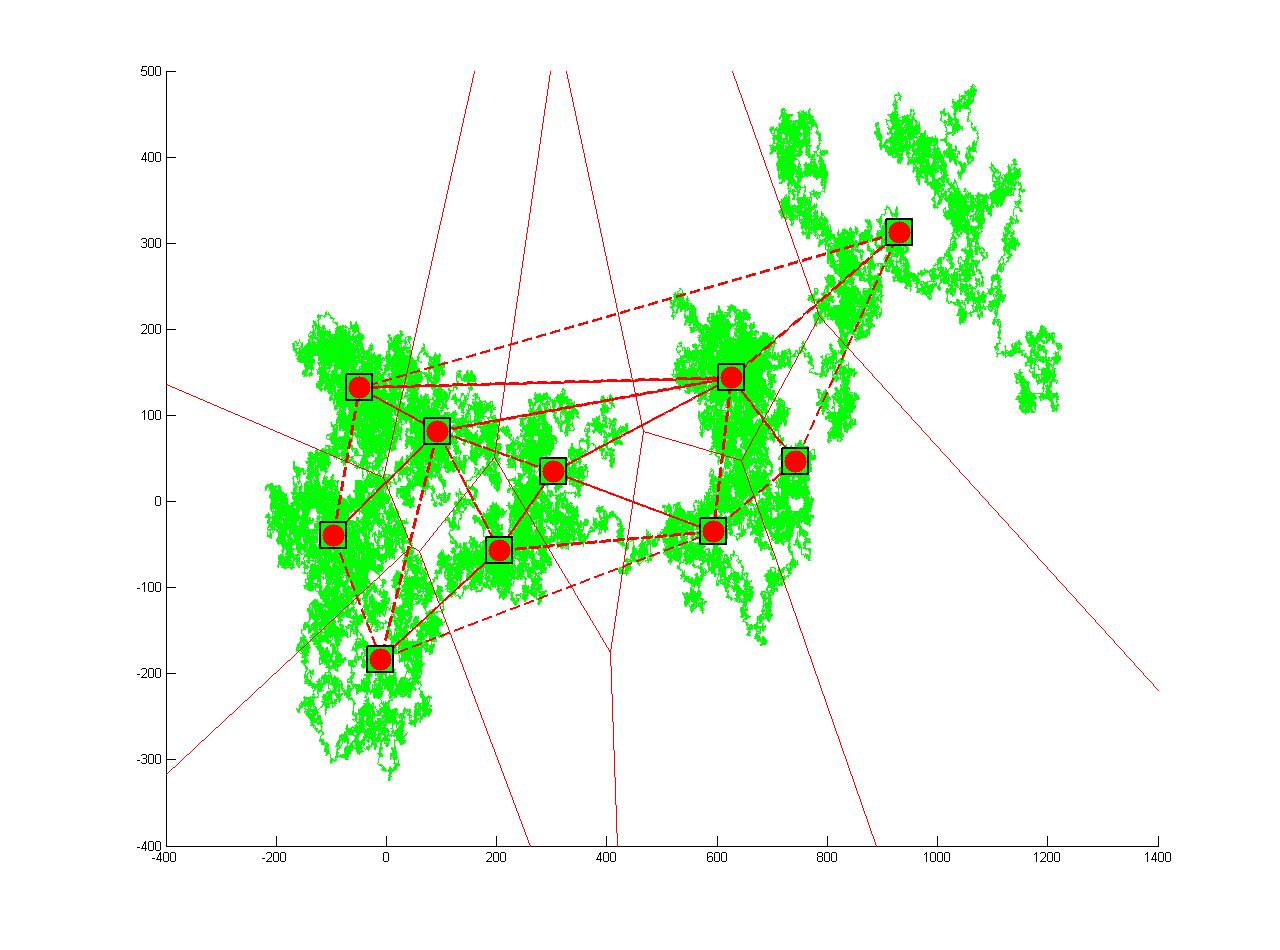
\includegraphics[width=8.0cm,height=8.0cm]{Figures/ClusteringRW/rw_1000000_delauney_kmens_convex_hull_voroni_onKM.jpg}


\section{The Matrix Exponential}
The matrix exponential of a matrix $\mat{A}$ is defined as
\begin{align*}
  e^{\mat{A}}
  &= \mat{I} + \mat{A} + \frac{\mat{A}^2}{2!} + \dots \\
  &= \sum_{k = 0}^\infty \frac{\mat{A}^k}{k!}.
\end{align*}

The Pade approximation to
$e^{\mat{A}}$ is
\begin{displaymath}
  e^{\mat{A}} \approx R(\mat{A}),
\end{displaymath}
with
\begin{align*}
  R_{pq} (\mat{A})
  &= (D_{pq}(\mat{A}))^{-1} N_{pq}(\mat{A}) \\
  \intertext{where}
  D_{pq}(\mat{A})
  &= \sum_{j=1}^p \frac{(p+q-j)! p!}{ (p+q)!j!(p-j)!}\, \mat{A}^j \\
  \intertext{and}
  N_{pq}(\mat{A})
  &= \sum_{j=1}^q \frac{(p+q-j)! q!}{ (p+q)!j!(q-j)!}\, \mat{A}^j.
\end{align*}
See \cite{Moler78nineteendubious} for a detailed accounting of this and other matters regarding the calculation of the matrix exponential.
%\citet{Moler78nineteendubious} \citep*{Moler78nineteendubious} \citep{Moler78nineteendubious} \citet*{Moler78nineteendubious}


\chapter{Software}

Computers are getting more powerful over time but size of the problems we're solving scales with the increased performance. Tools for acquiring and storing data are improving at an even faster pace than processors.  It turns out the communication is the real bottleneck to scaling many algorithms. The capacity of fast memory close to the computing resource (cache) grows very slowly in time.


\section{BLAS }

\section{Atlas}

\section{MKL}

\section{fftw}

\section{Graphviz - Graph Visualization Software}
Graphviz ( http://www.graphviz.org ) is open source graph visualization software. Graph visualization is a way of representing structural information as diagrams of abstract graphs and networks. It has important applications in networking, bioinformatics,  software engineering, database and web design, machine learning, and in visual interfaces for other technical domains.

Graphviz is used to generate collaboration, inheritance, and call diagrams the KL documentation. There is an API that is used in the KL framework to facilitate graph visualization.

\section{ARPACK}
ARPACK++ is an object-oriented version of the Fortran ARPACK package. ARPACK is designed to compute a few eigenvalues and eigenvectors of large scale sparse matrices and pencils via the Arnoldi process for finding eigenvalues called. These methods utilize Krylov Subspace Projections for iterative solution that avoids matrix multiplication.  ARPACK implements the implicit restarted Arnoldi method which reduces the storage requirements of the traditional Lanczos iteration for Hermitian matrices and Arnoldi iteration for general matrices.  The key to the Krylov method is to calculate the linear subspace of $\Real^{(n,n)}$ induced by span of the first m powers of the image of $b$ under a linear operator $A$, $\kappa_m(A,b) | A \in \mathbb R^{(n,n)}
b\ in \mathbb R^n = \{b, Ab (A)^2b, \ldots (A)^mb \}$.  This avoids direct matrix matrix operations when finding the first few eigenvector, eigenvalue pairs in a large system of linear
equations.

\section{ATLAS}
Automatically Tuned Linear Algebra software.

\section{METIS}
METIS is a software library for finite element analysis and graph partitions.  It also can be used to reduce the fill order of
sparse matrices.


\section{SDPA}
SDPA is a software library for solving SDPs using on the Mehrotra-type predictor-corrector infeasible primal-dual interior-point method. It is implemented C++ language and utilizes the machine dependent BLAS such as Intel MKL, ATLAS. LAPACK routines are used for matrix computations.  Efficient methods to compute the search directions exploiting the sparsity of the data matrices are implemented. Sparse or dense Cholesky factorization for the Schur complemetn matrix is automatically selected. The calculation of the Schur complement
matrix is implemented in reentrant code. A sparse version of SDPA is available that uses METIS and SPOOLES libraries for finding a proper sparse structure of the problem.

\section{SPOOLS}
SPOOLES is a library for solving sparse real and complex linear systems of equations. SPOOLES can factor and solve square linear systems of equations with symmetric structure, and it can compute multiple minimum degree, generalized nested dissection and multisection orderings of matrices with symmetric structure.  SPOOLES utilizes a variety of Krylov iterative methods. The preconditioner is a drop tolerance factorization.

\section{SuperLU}
SuperLU ( http://crd-legacy.lbl.gov/~xiaoye/SuperLU/) is a general purpose library for the direct solution of large, sparse, nonsymmetric systems of linear equations on high performance machines. The library is written in C and is callable from either C or Fortran. The library routines will perform an LU decomposition with partial pivoting and triangular system solves through forward and back substitution. The LU factorization routines can handle non-square matrices but the triangular solves are performed only for square matrices. The matrix columns may be preordered (before factorization) either through library or user supplied routines. This pre-ordering for sparsity is completely separate from the factorization. Working precision iterative refinement subroutines are provided for improved backward stability. Routines are also provided to equilibrate the system, estimate the condition number, calculate the relative backward error, and estimate error bounds for the refined solutions.

\section{SuiteSparse}
Tim Davis' ( http://www.cise.ufl.edu/~davis/welcome.html) collection of sparse matrix software.  Tim is also the curator of The University of Florida Sparse Matrix Collection (http://www.cise.ufl.edu/research/sparse/matrices/) a must see for anyone interested in sparse
matrices and visualization.

AMD: symmetric approximate minimum degree
BTF: permutation to block triangular form
CAMD: symmetric approximate minimum degree
CCOLAMD: constrained column approximate minimum degree
COLAMD: column approximate minimum degree
CHOLMOD: sparse supernodal Cholesky factorization and update/downdate
CSparse: a concise sparse matrix package
CXSparse: an extended version of CSparse
KLU: sparse$ LU$ factorization, for circuit simulation
LDL: a simple $LDL^T$ factorization
UMFPACK: sparse multifrontal $LU$ factorization
RBio: MATLAB toolbox for reading/writing sparse matrices
UFconfig: common configuration for all but CSparse
SuiteSparseQR: multifrontal sparse $QR$

\subsection{AMD}
AMD is a set of routines for pre-ordering a sparse matrix prior to numerical factorization. It uses an approximate minimum degree ordering algorithm to find a permutation matrix P so that the Cholesky factorization $PAP^\dag =LL^\dag$ has fewer (often much fewer) nonzero entries than the Cholesky factorization of A. The algorithm is typically much faster than other ordering methods and minimum degree ordering algorithms that compute an exact degree . Some methods, such as approximate deficiency [Rothberg and Eisenstat 1998] and graph-partitioning based methods [Hendrickson and Rothberg 1999; Karypis and Kumar 1998; Pellegrini et al. 2000; Schulze 2001] can produce better orderings, depending on the matrix. The algorithm starts with an undirected graph representation of a symmetric sparse matrix . Node $i$ in the graph corresponds to row and column i of the matrix, and there is an edge $(i,j)$ in the graph if $a_{ij}$ is nonzero. The degree of a node is initialized to the number of off diagonal non-zeros in row $i$, which is the size of the set of nodes adjacent to $i$ in the graph.

\subsection{UMFPACK}
UMFPACK is a set of routines for solving systems of linear equations, $Ax = b$, when $A$ is sparse and unsymmetric. It is based on the Unsymmetric-pattern MultiFrontal method. UMFPACK factorizes $PAQ$, $PRAQ$ and $PR^{-1}AQ$, into the product $LU$, where $L$ and $U$ are lower and upper triangular, respectively, $P$ and $Q$ are permutation matrices, and $R$ is a diagonal matrix of row scaling factors (or $R = I$ if row-scaling is not used). Both $P$ and $Q$ are chosen to reduce fill-in (new nonzeros in $L$ and $U$ that are not present in $A$). The permutation $P$ has the dual role of reducing fill-in and maintaining numerical accuracy (via relaxed partial pivoting and row interchanges). The sparse matrix $A$ can be square or rectangular, singular or non-singular, and real or complex (or any combination). Only square matrices $A$ can be used to solve $Ax = b$ or related systems. Rectangular matrices can only be factorize 
\chapter{Appendix Statistics}

\section{Concepts from Mathematical Statistics}The sampling distribution of an estimator is the probability distribution of the estimator under repeated sampling.  The standard error of a measurement is essentially the standard deviation of the process by which the measurement was generated.  When the underlying probability distribution of the generating process is known the standard error can be used to calculate confidence intervals.  Otherwise Chebyshev's inequality can be used. The standard error of a sample from a population is the standard deviation of the sampling distribution and may be estimated as $\frac{\sigma}{\sqrt{n}}$

Completeness is the ability of a statistical estimator to ensures that the parameters of the underlying probability distribution representing the model can be estimated from the statistic

Consider a family of probability distributions for a random variable $X$ parameterized by a parameter $\theta$. A quantity $T(X)$ that depends on the random variable $X$ but not on the parameter $\theta$ is called a statistic.  A statistic that captures all of the information in X that is relevant to the estimation of $\theta$ is called a sufficient statistic. Since the conditional distribution of $X$ given $T(X)$ does not depend on $\theta$, neither does the conditional expected value of $g(X)$ given $T(X)$. The conditional expected value is itself a statistic and so is available for use in estimation. If $g(X)$ is anestimator of $\theta$, then typically the conditional expectation of $g(X)$ given $T(X)$ is a better estimator of $\theta$. The Rao-Blackwell theorem makes this precise.


\section{L-Estimators \& M-Estimators}Order statistics of a sample ${X_i}$ can be used to estimate quantiles. An L statistic is a linear combination of an order statistic.  L statistics are used in Box plots.  An M-Estimator is the minima of sums of functions of the sample data.  Maximum Likelihood and Least Squares are examples of M-Estimators.


\section{Testing for normality and other distributions } Powerful inference methods can be employed when data is generated by a Gaussian process. This section describes techniques for testing the normality of a sample and comparing two samples.  Kolmogorov-Smirnov test uses the fact that the empirical cumulative distribution function is normal in the limit. It is a non-parametric and distribution free test. Given the empirical distribution
 \[F_n(x) = \frac{1}{n} \sum\limits_{n}^{i=1} \biggl\{\begin{array}{c}1 :x_i\leq x \\0 : x_i>x\\ \end{array}\]
 , and a test CDF\[ F(x)\] the K-S test statistics are $D_n^+ = max(F_n(x)-F(x) ) $ and $D_n^- = min(F_n(x)-F(x) )$ The generality of this test comes at a loss in precision near the tails of a distribution.  The K-S statistics are more sensitive near points close to the median, and are only valid for continuous distributions.  The Kuipers test uses the statistic $D_n^+ + D_n^- $ and is useful for detecting changes in time series since the statistic is invariant in ???? transformation of the dependent variable $ F_n$.  The Anderson-Darling test is based on the K-S test and uses the specific distribution to specify the ????critical values??? of the test.  The chi-squared is based on the sample histogram and allows comparison against a discrete distribution, but has the potential drawback of being sensitive to how the histogram is binned and requires more samples to be valid.  The Shapiro-Wilk test uses the expected values of the order statistics of $F(x)$ to calculate the test statistic.  It is sensitive to data that are very close together, and numerical implementations may suffer from a loss of accuracy for large sample sizes.

 K-S [Chakravarti, Laha, and Roy, (1967). Handbook of Methods of Applied Statistics, Volume I, John Wiley and Sons, pp. 392-394].  Shapiro-Wilk [Shapiro, S. S. and Wilk, M. B. (1965). "An analysis of variance test for normality (complete samples)", Biometrika, 52, 3 and 4, pages 591-611.]


\section{Regression Methods}Standard least squares regression consists in fitting a line through the data points (training points in learning theory) that minimizes the sum of square residuals.  The underlying assumption is that the data and the response can be modeled by a linear relationship.  In the event that the model accurately captures the functional dependence of the response generated by the data, and under the assumptions that the data is corrupted by Gaussian noise, precise statistical inferences can be made on the model parameters.  Modifications to this standard model include nonlinear mapping of the input data, local fitting, biased estimators, subset selection, coefficient shrinking, weighted least squares, and basis expansion transformations.

The multiple regression model in matrix notation can be expressed
as
(BBCREVISIT)

These equations hold for the univariate and the multivariate case.

$\textbf{Y} = \textbf{X}{\beta} + \textbf{e}$.

where $\textbf{e} =_d N(\mathbf{\mu},mathbf{\Sigma})$

$E \textbf{Y} = mathbf{\mu} X mathbf{\beta}$

$var \textbf{Y} = \sigma^2 \textbf{I}$

Maximum Likelihood and Least Squares give same estimator;

$\widehat{mathbf{\beta}}=(X^TX)^{-1} X^T Y$

$\hat{\sigma}^2 = frac{1}{n} || Y- \hat{\mu} ||^2$

Multivariate regression is the extension to $YM = Xb + e$

Here $Y, X, b$, and $e$ are as described for the multivariate regression model and $M$ is an $m x s$ matrix of coefficients defining linear transformation of the dependent variables. The normal equations are $X'Xb = X'YM$ and a solution for the normal equations is given by $b = (X'X)-X'YM$. Here the inverse of $X'X$ is a generalized inverse if $X'X$ contains
redundant columns.




\section{Generalized Linear Models}Suppose we have $n$ observations of $k$ dimensional data denoted $\{x_i\}_{i=1}^{k}$ and for each observation we have a response $y_i$. We wish to fit the observations to the responses. Generalized Linear Regression is a modeling technique that allows for non normal distributions and models non-linear relationships in the training data. M-estimators are used to fit a generalized linear model Ref Huber (1964).
A linear model $ Y =\Lambda(X)=X\beta + \epsilon$ fits a linear relationship between the dependent variables $Y_i$ and the predictor variables $X_i$ \begin{equation}Y_i=\Lambda(X_i)=b_o + b \circ X_i.\end{equation}
A generalized linear model $Y= g(\Lambda(X) ) + \epsilon $ fits the data to $ Y = g (X \circ W)$. Fitting the model consists of minimizing the objective function $\sum\limits_{i=1}^{n} g(e_i)=\sum\limits_{i=1}^{n} g(y_i- x_i \beta)$
, where $e_i$ are the residuals $y_i-x_i \beta$. We see that for ordinary least squares $g(e_i)=e_i^2$, and the usual matrix equations fall out by differentiating with respect to $\beta$. Carrying this out for general $g$ \begin{equation} \sum\limits_{i=1}^{n} \frac{\partial  g(y_i-x_i \beta)}{\partial \beta}=0 \end{equation} gives the system of $k+1$ equations to solve for estimating the coefficients $b_i$.  If we set$\alpha(x)=\frac{g'(x)}{x}$ and calculate the derivative above, we have to solve \begin{equation} \sum\limits_{i=1}^{n} \omega(e_i) (y_i-x_i \beta) x_i = 0 \end{equation}. Which gives rise to a weighted least squares where the weights depend on the residuals - which depend on the coefficients - which depend on the weights.  This suggests an iterative algorithm; \begin{equation} \beta^\tau = ( X^{t} W^{(\tau-1)} X )^{-1} X^{t} W^{\tau-1} y \end{equation} where $W_{ij}^{(\tau-1)}=\alpha(e_{i}^{(\tau-1})$.  Several parameterizations are popular for the exponential family. The most general form of the distribution \[ p(x,\theta) = f(x,\theta)e^{g(x,\theta)} \in C^2(\dblr \otimes \dblr ) \otimes C^2(\dblr \otimes \dblr )\].  The estimators derived below assume that $f$ and $g$ are separable, \[ p(x,\theta) = f(x) h(\theta) e^{\alpha(x) \beta(\theta)} \in C^2(\dblr) \otimes C^2(\dblr ) \otimes C^2(\dblr ) \otimes C^2(\dblr ) \].  From \[ \int\limits_{x=-\infty}^{x=+\infty} p(x,\theta) dx \: =1\] we get \[ \fderiv{\theta}{p(x,\theta)} = 0 = \sderiv{\theta}{p(x,\theta)}d \] Since the parametrization we have chosen for the exponential family allows, in the sequel we drop the notation for dependent variable and denote the derivative with a prime. \[ \fderiv{\theta}{p(x,\theta)} = \fderiv{\theta}{f h e^{\alpha \beta}} = h' f e^{\alpha \beta} + f h \alpha \beta' e^{\alpha \beta} = \bigl( \frac{h'}{h} + \alpha \beta' \bigr) p(x,\theta) \] which gives \[\int \fderiv{\theta}{p(x,\theta)} dx = \int \bigl( \frac{h'}{h} + \alpha \beta' \bigr) p(x,\theta) dx= \frac{h'}{h} \int p(x,\theta) dx \:+\: \beta' \int \alpha(x) p(x,\theta) dx = \frac{h'}{h}+\beta' E[\alpha(x)] \] so that \[E[\alpha(x)]=-\frac{h'}{h \beta'}\]. Continuing along this vein,\begin{gather*} 0 =\int \sderiv{\theta}{p(x,\theta)} dx = \int \fderiv{\theta}{\bigl( \frac{h'}{h} + \alpha \beta' \bigr) p(x,\theta) } dx =\\  \int \bigr(\frac{h''}{h}-\frac{(h')^2}{h^2}+\alpha \beta'' \bigl ) p(x,\theta) + (\frac{h'}{h}+\alpha \beta') \fderiv{\theta}{p(x,\theta)} \: dx = \\ \int \bigr(\frac{h''}{h}-\frac{(h')^2}{h^2}+\alpha \beta'' \bigl ) p(x,\theta) + (\frac{h'}{h}+\alpha \beta')^2 p(x,\theta) \: dx = \\ \int \bigr(\frac{h''}{h}-\frac{(h')^2}{h^2}+\alpha \beta'' \bigl ) p(x,\theta) + (\frac{h'}{h}+\alpha \beta')^2 p(x,\theta) \: dx = \\ \int \bigr(\frac{h''}{h}-\frac{(h')^2}{h^2}+\alpha \beta'' \bigl ) p(x,\theta) + (\alpha \beta'- E[\alpha(x)]\beta')^2 p(x,\theta) \: dx \end{gather*}  Keeping in mind that  \[ Var[a x ]= E[ (ax-E(ax)^2 ] = a^2 E [ (x-E[x])^2] =a^2 Var[x]  \]  we get the variance via\[ \bigr(\frac{h''}{h}-\frac{(h')^2}{h^2}+E[\alpha(x)] \beta'' \bigl )+ Var[\alpha(x) \beta'(\theta)] = \bigr(\frac{h''}{h}-\frac{(h')^2}{h^2}+E[\alpha(x)] \beta'' \bigl )+ (\beta')^2 Var[\alpha(x)] = 0 \]  The score $U(x)$ is given by \[ U(x)=\pfderiv{\theta}{L(\theta,x)} = \pfderiv{\theta}{\log \: p(x,\theta)}=\pfderiv{\theta}{\bigr( \log h(\theta) + \log f(x) + \alpha(x) \beta(\theta)\bigl) } = \frac{h'}{h} + \alpha \beta'\] so \[E[U(x)]=\beta'E[\alpha(x)] + \frac{h'}{h} =0 \].  The Fisher Information $\mathcal{F}$ is defined \[\mathcal{F}=Var[U(x)] =Var[ \alpha \beta' + \frac{h'}{h}]= Var[ \alpha \beta'] \] So from above we have \[Var[U(x)]= Var[ \alpha \beta'] =\bigr(-\frac{h''}{h}+\frac{(h')^2}{h^2}-E[\alpha(x)] \beta'' \bigl )\].  Now differentiating,  \[ \fderiv{\theta}{U(\theta,x)} = \frac{h''}{h} - \frac{(h')^2}{h^2} + \alpha \beta''\] \[E[U'(\theta,x)]=\frac{h''}{h} - \frac{(h')^2}{h^2} + E[\alpha] \beta'' =  \frac{h''}{h} - \frac{(h')^2}{h^2} -\frac{ \beta'' h'}{\beta'}= - Var[U(x)] \].  Note that if we write the parametrization of the separable exponential family as \[ p(x,\theta) =  e^{\alpha(x) \beta(\theta)+\log(f(x))+\log(h(\theta))}\] then, \[\sderiv{\theta}{\log(h(\theta))}=\fderiv{\theta}{\frac{h'}{h}}=\frac{h''}{h}-\frac{(h')^2}{h^2}\].     (BBCREVISIT - this duplicates and has notation clash with material above).

A general form of the exponential distribution \begin{equation} \rho(x;\theta) = exp( \frac{x \theta - \xi(\theta) }{\sigma} ) \nu ( x) \end{equation} has a log likelihood for a random sample $\{ X_i  \}_{i=1 \hdots N}$ given functionally by \begin{equation} \mathcal{L} (\theta) =  \sum\limits_{i=1}^{N} [ X_i  \theta  - \xi (\theta) + log   ( \nu ( X_i ) ) ] \end{equation} The scale parameter $\sigma$ and $\theta$ are orthogonal parameters in that E [ ] The Generalized Linear model can  $\rho'$ is referred to as a link function in the statistical literature.  If $\rho'(x)= x\field(1)$ and $\epsilon=(\epsilon_1, \hdots ,\epsilon_n)$ are iid $N(\mu,\sigma)$ we have multiple linear regression.  In classification problems or binomial models the logit $\rho'(x)=log(x/(1-x))$ link function is used. The logit is extended to the $k$ category case by \begin{equation}\rho'( x_i | x_j j \neq i)= log ( \frac{x_i}{1- \sum\limits_{j \neq i} x_j})\end{equation}. The posterior probability densities ${p_i(?)}$ bbcrevisit (or $p_i$ the probability of observing class $i$)  of k classes are modeled by linear functions of the input variables $x_i$.



\section{Fitting the GLM}Iteratively re-weighted least squares (IRLS) is used to for fitting generalized linear models and in finding M-estimators.  The objective function

\begin{equation}
J(\beta^{i+1}) = arg min \sum w_i ( \beta) | y_i - f_i (\beta) |
\end{equation}

is solved iteratively using a Gauss-Newton or Levenberg-Marquardt (LM) algorithm. LM is an iterative technique that finds a local minimum of a function that is expressed as the sum of squares of nonlinear functions. It is a combination of steepest descent and the Gauss-Newton method. When the current solution is far from the minimum the next iterate is in the direction of steepest descent. When the current solution is close to the minimum the next iterate is a Gauss-Newton step.

Linear least-squares estimates can behave badly when the error is not normal.  Outliers can be removed, or accounted for by employing a robust regression that is less sensitive to outliers than least squares.  M-Estimators introduced by Huber generalize maximum likelihood estimation and are less biased and more efficient.  Instead of trying to minimize the log likelihood

\begin{equation}
L(\theta) = \sum - log ( p(x_i, \theta)
\end{equation}

Huber proposed minimizing

\begin{equation}
M(\theta) = \sum  \rho(x_i, \theta)
\end{equation}

where $\rho$ reduces the effect of outliers. Common loss function are the Huber, and Tukey Bisquare.  For $\rho(x) = x^2$ we have the familiar least squares loss.

M estimators arise from the desire to apply Maximum Likelihood Estimators to noisy normal data, and to model more general distributions. They provide a regression that is robust against outliers in the training set, and allow for modeling of non-Gaussian processes. When $\rho$ above is a probability distribution, we are preforming a maximum likelihood estimation.

The Huber function which is a hybrid $L^2$ $L^1$ norm
\begin{equation}
\rho_\eta(e_i)=\biggl\{\begin{array}{cc}
\frac{e_i^2}{2} & |e_i| \leq \eta \\
  \eta |e_i| - \frac{\eta^2}{2} & |e_i| > \eta \\
\end{array}
\end{equation}
The  Tukey Bisquare estimator is given by
\begin{equation}
g_\eta(e_i)=\biggl\{ \begin{array}{cc} \frac{\eta^2}{6} (
1-[1-\frac{e_i}{\eta}_2]^3) & |e_i| \leq \eta \\
\frac{\eta^2}{6} & |e_i| > \eta \\
\end{array}
\end{equation}

Numerical procedures for doing this calculation are the Newton-Raphson method [see the section on root finding below ], and Fisher-Scoring method [ replace $ \frac{\partial^2 \mathcal{L}(\mathbf{\theta})}{\partial \mathbf{\theta} \partial \mathbf{\theta}^{t} }$ with $E[ \frac{\partial^2 \mathcal{L}(\mathbf{\theta})}{\partial \mathbf{\theta} \partial \mathbf{\theta}^{t} }  ]$. For high dimensional data, many models may be fit in an attempt to find the simplest one that can explain the data.  In the language of statistical learning theory, the choice of a norm $\rho$ is tantamount to choosing a loss function. Restricting the admissible functions to the one parameter family of exponential probability distributions defines the capacity via a functional form of the law of large numbers. \cite{Scholkopf B. (2002)}



\section{Feature Subset Selection (FSS)}The goal of feature selection techniques to to improve the model building process by eliminating features that do not have discriminative power. Algorithms for feature selection either rank features or create subsets of increasing optimality.  FSS should be contrasted with feature extraction techniques such as PCA, LLE, or Laplacian eigenmaps.  The goal of feature extraction is to transform data from a high dimensional space to a low dimensional one while preserving the relevant information.

The statistical approach to feature selection most commonly used is stepwise regression.  Common optimality criteria are FSS schemes the Kolmogorov-Smirnov Test ,the t-test, the f-test, the Wilks Lambda Test and Wilcoxon Rank Sum Test.

It's important to distinguish the FSS process from a data dimension reduction process such as PCA which requires all the original measurements to compute the projection. The better FSS algorithms are recursive

Construct a $p x M$ basis matrix $H^{T}$ and transform feature vector $x' = H^{T} x$.


Generalize to $L^{2}$ with smoothing splines

Smoothing spline $RSS(f,\lambda)= \sum\limits_{i=1}^{N} (y_{i} -f(x_{i}) )^{2} + \lambda \int f''(t)^{2} dt$. where $f \in C^{2}(\field{R} )$ This is minimized in $L^{2}$ the first term measuring closeness of fit, and the second term penalizes curvature. $\lambda \rightarrow 0$ gives any function interpolating the data points ${x_i}_{i  \in {1, ... N} } $ an $\lambda \rightarrow \infty$ constrains $f$ to be linear.

\section{Longitudinal Data Analysis} Longitudinal data analysis is the observation of multiple subjects over repeated intervals. Binary repeated responses are typically modelled with a marginal or random effects model, which will be made precise below. Marginal Models are a generalization of the GLM presented above for correlated data.  Here, the correlation is inter subject across time.  Statistical analysis of longitudinal data must take into account that serial observations of a subject are likely to be correlated, time may be an explanatory variable, and that missing response data my induce a bias in the results.  Let ${X_{ij}}$ be time varying or fixed covariates for the binary response ${Y_{ij}}$ of subject $i \in {1,...n}$ at time intervals $j \in {t_1,...t_m}$. By convention $X_{ij} \in \field{R} x \field{R^p}$ where the first dimension is the intercept. The marginal model is; $logit (E(Y_{ij} | X_{ij}) ) = X_{ij}^{\dagger} \beta$ and enforces the assumption that the relationship between the covariates and the response is the same for all subjects. Recall that for a binary response, $E(Y_{ij} | X_{ij}) = P(Y_{ij}=1 | X_{ij})$.  The random effects model takes into account that the relationship between the covariates and response varies between subjects; $logit (P(Y_{ij}=1 | X_{ij}) ) = X_{ij}^{\dagger} \beta_i$ If it is know that only a subset of the covariates are involved in the inter-subject variability, we can set $\beta_i= \beta + \beta_i$ and write $logit (P(Y_{ij}=1 | X_{ij}, \beta_i) ) = X_{ij}^{\dagger} \beta + O X_{ij} \beta_i$ Where the kernel of $O : \dblr^n \rightarrow \dblr^{n'}$ is the span of the covariates that do not change between subjects.  If $\lambda_i =_d N(0,\sigma)$ then the difference in the parameter vectors $\beta$ in the two models differ according to $\sigma$.

The GEE method of fitting the marginal model is described in: \cite{Liang, K-Y and Zeger, S. L.(1986)}  The Survival Analysis is a form of longitudinal analysis that takes into consideration the amount of time an observation is made on a subject.  GLM's can be used to fit discrete longitudinal hazard models derived from survival analysis, see  \cite{Prentice and Gloeckler (1978)}.   \cite{Meyer, B.D. (1990)} generalized that approach to account for an unobserved subject heterogeneity.  \cite{Holmen, M (2005)} applied the hazard model of \cite{Prentice, R. and L. Gloeckler (1978)} to the takeover hazard of large firms.  A negative relationship between dual class ownership and value is empirically known, and that relationship can be explained by the lower takeover probability of the dual class firms.  Dual class entities had a higher risk for takeover, but the hazard is lower since these firms use the dual class structure to change the capital structure in a way that allows the controlling shareholders to remain in control by reducing firm value.  The proportional hazards model can be discretized, but it is important to identify whether the process is truly a discrete process.  In that case the link function should be the logit as the Marginal Model above specifies, rather than the log-log function of the discretized proportional model.  The difference is the modelling of a probability transition in the former case versus a rate for the latter case.  Variable selection techniques for longitudinal data are relatively limited and most seem to rely on Wald type tests. Wald tests to include a variable are based on already computed maximum likelihood values. The Rao score test is used to include a covariate in the model building process.  The Wald test calculates \[z^2=\frac{\widehat{\beta}}{stderr}=_d  \chi^2\]  The likelihood ratio statistic for comparing two models $L_0 \in L_1$ \[-2 \frac{L_0}{L_1} =_d \chi^2\] is useful for backward stepwise variable subset selection. The degrees of freedom of the of the statistic is equal to the difference in dimension of the two models.


\section{Discretization \& Sheppard's Correction}W. Sheppard (1898) Derived an approximate relationship between the moments of a continuous distribution and it's discrete approximation. This provides a transformation to statistical estimators that correct for the binning of continuous data.  As the scale at which datum are collected is increased, the variance of an estimate can become biased.  It is important to assess  bias caused by grouping and to correct it if necessary. The  bias of the approximate maximum likelihood estimator where observations are approximated by interval midpoints $O(w^2)$, where $w$ is the bin width. A Sheppards correction can be used to reduce the bias to order $O(w^3)$,  Signal processing engineers often have to deal with such a quantization effect when designing finite precision systems, image processing being a particularly relevant example. The engineering community typically models the quantization noise $Q=[X]-X$, where $[X]$ is the quantized realization of $X$. One might be tempted to apply a Sheppard's correction to the moments of the quantized data, thinking that $Var(X)<Var([X])$ but it is possible to construct examples where $Q$ and $[X]$ are independent, or where $Cov(X,Q)$ is such that $Var(X)>Var([X])$.  Shepard's correction is limited in that is doesn't apply to the first moment, and the frequencies of the first and last bins need to be low.  Expand $p(x;\theta)$ in a Taylor series and substitute in the Maximum Likelihood equations. \cite{Lindley, D. V. (1950)}  Suppose we have n realizations of iid RV's ${X_1, \hdots , X_n}$ and the data is collected on a discrete grid on the range of $X$ $Ran(X)=\{[y_i-d_i/2,y_i+d_i/2]\}_{i=1}^{i=m}$ where the intervals are centered on the location where a measurement. The realized values ${y_1, \hdots , y_m}$ have probabilities $p_i=\int\limits_{y_i - d_i /2}^{y_i+d_i /2} p(x;\theta) \;\; dx$ Expanding $p(x;\theta)$ in a Taylor series about $y$, $p(x;\theta)= \sum\limits_{i=0}^{\infty} \frac{p^{(i)}(y) }{i!} (x-y)^i$.


\section{Multidimensional Scaling}Multidimensional scaling (MDS) is an alternative to factor analysis. The aim of MDS and factor analysis is to detect meaningful underlying dimensions that explain similarities or dissimilarities data points. In factor analysis, the similarities between points are expressed via the correlation matrix. With MDS any kind of similarity or dissimilarity matrix may be used.  Given $n$ observations ${x_i}_{i=1}^{n} \in \dblr^k$ and $n^2$ distances $d_{ij}$ between them, MDS looks for $n$ points ${\xi_i}_{i=1}^{n}$ in $dblr^l : l<k$ that preserve the distance relations. When a metric $\rho()$ exists for the similarity measure, gradient descent is used to minimize the MDS functional $S(\xi_1, \ldots , \xi_l)=\biggl( \sum_{i \neq j} d_{ij}-||\xi_i-\xi_j||_{\rho}\biggr)^\frac{1}{2}$.


\section{Principal Components} For a data set $\textbf{X} \in
M_{(N,m)}(\mathbb{R}) = { x_1, x_2, \ldots x_N | x_i \in
\mathbb{R}^m } $, the first k principal components provided the
best k dimensional linear approximation to that data set.
Formally, we model the data via $f(\theta) = \mu + \textbf{V}_k
\theta | \mu \in \mathbb{R}^m, V_k \in O_{m,k}(\mathbb{R}),
\theta \in \mathbb{R}^k$ so $f(\theta)$ is an affine hyperplane
in $\mathbb{R}^m$


\section{Evaluating classifier performance} Multi-class problems can be treated simultaneously or broken in to a sequence of two class problems.  Cross validation is used both for classifier parameter tuning and for feature subset selection.  Student-t and ANOVA can be used to evaluate the performance of classifiers against one another.  The Student-t test compares two classifiers, while the ANOVA test can compare multiple classifiers against one another.  Confusion matrices and ROC graphs are commonly employed visualization tools for assessing classifier performance. The rows of a confusion matrix add to the total population for each class, and the columns represent the predicted class.  An ROC curve plots the TP rate against the FP rate. Often a curve in ROC space is drawn using classifier parameters for tuning purposes.

\begin{table}[h]
\begin{tabular}{|c|c|}
  \hline
  % after \\: \hline or \cline{col1-col2} \cline{col3-col4} ...
  TN &  FP \\
  \hline
  FN & TP \\
  \hline
\end{tabular}
\caption{Two class confusion matrix where the proportions are
specified}
\end{table}

Common performance metrics for the two class problem are sensitivity (TP), specificity (TN), precision (the proportion of predicted cases within a class that were correct), and accuracy (the overall proportion of correct predictions). These metric can be extended to more than two classes by defining $A=tr ( C ) / || C ||_{L^\infty}$ where $C$ is the confusion matrix. TP, FN, FP, TN are proportions defined for the two class problem.


\section{Covariance Matrix Estimation } For numerical stability in regression algorithms, the covariance matrix needs to be positive definite.  An well conditioned estimator for the covariance matrix of a process can be obtained by mixing the sample covariance with the identity matrix.  This is a linear shrinkage estimator based on a modified Frobenius norm for $A \in M_{mn}$  \begin{equation} ||\mathbf{A}||_{\cal{F}}= \sqrt{ \frac{tr (A A^t)}{n}} \end{equation}  Without loss of generality, set $\mu =0$ and let $\widehat{\Sigma} = \alpha \mathbb{I} + \beta \mathbf{S}$ where $\mbf{S}=\frac{\mbf{X}^T \mbf{X}}{n}$ is the sample covariance.  We seek to minimize $E( ||\widehat{\Sigma} - \Sigma||^2)$, but since we don't know the true population covariance matrix, we have to form an approximation.

Many applications in statistics and machine learning require an estimate of the covariance matrix or it's inverse. Generally we avoid taking inverses of matrices in practice for stability reasons. The sample covariance matrix usually performs poorly as a proxy for the underlying covariance matrix.  There is a large literature on this subject; particularly fomr the finance industry where this is an important part of portfolio theory.two major challenges in covariance estimation are the positive-defniteness constraint and the high-dimensionality where the number of parameters grows quadratically in the dimension.

\section{Testing For Normality}In this section we will use the term $EPDF_X$ to mean the empirical probability density function. There are a variety of univariate tests to help determine which parametric distribution your data belongs to. These fall under the category of Goodness of Fit testing. For a parametric family the null hypothesis $H_o : X=_d p(x| \theta)$ is tested against the alternative that $X$ does not belong to the family $p(x|\theta)$ There are also family of test to determine whether two $EPDF$'s come from the same distribution.  Keep in mind that there are many transformations ( polynomial, logarithmic, \& rational )  to transform data to look more Normal.  The presence of tails and skew will be the most problematic to deal with.

The Anderson-Darling test determines whether a sample comes from a specified distribution. The sample data can is transformed to a uniform distribution and then a uniformity test is then done on the transformed data. The test statistic is compared against pre-computed values for the assumed probability distribution.

The Kolmogorov-Smirnov is non-parametric a form of minimum distance estimation.  It can be used to test a sample against a reference or to compare two samples against each other.  In the one sided case the KS statistic calculates the distance between the $EPDF$ of a sample and a reference.  In the two sided case the distance between the $EPDS$'f of the two samples are calculated.  The KS test is robust to location and shape, making it  Omnibus tests evaluate whether the explained variance in a set of data is significantly greater than the unexplained variance. For example is the F-test in ANOVA. Omnibus tests of normality based on the likelihood ratio outperform the Anderson-Darling test statistic.


\chapter{Appendix Probability}

Let $\mu$ be a non-negative countably additive set function over a sigma algebra $\Omega$ of sets from a sample space $S$. In probability theory, $\Omega$ is the set of possible events $E$. Sets of measure zero denote impossible outcomes. An important feature of measures $\nu$ and $\mu$ that agree on sets of measure zero is the ability to define a derivative $\frac{d \nu}{d \mu}$, the Radon-Nikodym derivative.  When $\nu (E)=0 \fall E \in \Omega \;| \; \mu(e)=0$  Alternatively, given a measure $\mu$ and a nonnegative measurable function $f$, a new measure can be defined by $ \nu(E) = \int\limits{E \in \Omega}{} f d \mu$. A random variable is a real valued function on a sample space into a metric space, $X : S \rightarrow \dblr^{1} $. Associated with a random variable is it's probability density function $f_{X}(x)=P(\{s \in S | X(s) = x\})$ operating on an algebra of sets generated by the sample space $S$. By definition, $f_{X}(x)$ is the sum of probabilities of the events in $S$ that get mapped to $x \in \dblr$ by $X$.  Let $\script{B}(S)$ be the Borel sets on $S$, then $X$ has density $f$ if $P(X \in A) = \int_{A \in \script{B}(S)} f(x) dx $ and distribution function $F(x) = P(X<x)=\int\limits_{-\infty}^x f(y) dy$ so $F'(x)=f(x) \;\; a.e.$.  $E(X)=\int x f(x) dx$ is the expectation of $X$.  The characteristic function $\phi(x) = E(e^{itX} )$ determines the distribution and is used in the proof of the CLT theorem, testing for symmetry, and conditional independence.  We denote samples with lower case in this section.  $x_1 \ldots x_n$ is a random sample of size $n$  In $\dblr^n$ the random variate $X$ has distribution function $F(x_i, \ldots , x_n) = P(X_1<x_1, \ldots , X_n<x_n )$ and density $f(x_1, \ldots , x_n )$.

For parametric distributions, one is interested in the question of what value of a parameter best describes the data at hand.  This obviously requires the assumption that the data derives from a family of distributions parameterized by one or more variables $\theta_k$.  If $x_1 \ldots x_n$ is a random sample from $X$ with a distribution given by $p(x;\theta_1 \ldots \theta_k)$, we can think of the joint pdf of of the sample $L(x_i, \ldots,x_n) = \prod\limits_{i=1}^{n} p(x_i;\theta_1 \ldots \theta_k)$ as being explained by the parameters.  $L$ is the likelihood of the data given the parameters.  The maximum likelihood estimate is obtained by solving the set of equations;
\begin{eqnarray} \nonumber
  \frac{\partial L(\theta_1 \ldots \theta_k)}{\partial
  \theta_1}=0 \\ \nonumber
  \vdots \\ \nonumber
   \frac{\partial L(\theta_1 \ldots \theta_k)}{\partial
   \theta_k}=0 \\ \nonumber
\end{eqnarray}

%$ P(X), P(X|Y), P(X,Y) p(x) p_i x_i \mathbf{X} \mathbf{\beta}$

The statistical moments of a random variable $X$ are defined $\mu_n = E [ X^n] = \int_\Omega X^n P(X)dX$.  The characteristic function is the fourier transform of $P(X)$ \[\Phi(\omega)=\digamma \mathcal{F} [P(X)] (\omega) = \int\limits_{\infty}^{\infty} e^{i \omega X} P(X) dX.\]  Taking the logarithm and expanding in a MacLauren series, we can relate the statistical moments to the coefficients. Statistical moments are central or raw.

Common sample descriptive statistics relating to location, scale, tail size,  and peakedness;
\[ mean = \hat{\mu_1} = \frac{1}{n}\sum x_i  \]
\[ variance = sdd^2 =  \hat{\mu_2} = \frac{1}{n-1} \sum (x_i- \hat{\mu_1}\]
\[ skewness = \frac{ \hat{\mu_3}}{\hat{\mu_2}^{3/2}} \]
\[ kurtosis = \frac{\hat{\mu_4}}{\hat{\mu_2}^2} \]
The linear association between $X_i$ and $X_j$ is measured by the covariance \[ Cov_{ij} = \sigma_{ij} = \frac{1}{n-1} \sum_k (x_ki - \hat{\mu_1}_i)(x_{kj} - \hat{\mu_1}_j). \]  For a measure without dependence on units the scaled covariance is the correlation \[C_{ij} =\frac{\sigma_{ij}}{\sqrt{\sigma_{ii}}\sqrt{\sigma_{jj}}}\]

%

%sample and population central moments are related

%Joint

%Conditional

%Marginal
%Marginal -relating to or being a function of a random variable
%that is obtained from a function of several random variables by
%integrating or summing over all possible values of the other
%variables <a marginal probability function>

%Bias Variance Tradeoff of an estimator

The sampling distribution of an estimator is the probability distribution of the estimator under repeated sampling.  The standard error of a measurement is essentially the standard deviation of the process by which the measurement was generated.  When the underlying probability distribution of the generating process is known the standard error can be used to calculate confidence intervals.  Otherwise Chebyshev's inequality can be used. The standard error of a sample from a population is the standard deviation of the sampling distribution and may be estimated as $\frac{\sigma}{\sqrt{n}}$


%Sufficient
%In statistics, one often considers a family of probability
%distributions for a random variable X (and X is often a vector
%whose components are scalar-valued random variables, frequently
%independent) parameterized by a scalar- or vector-valued
%parameter, which let us call \theta. A quantity T(X) that depends
%on the (observable) random variable X but not on the
%(unobservable) parameter \theta is called a statistic. Sir Ronald
%Fisher tried to make precise the intuitive idea that a statistic
%may capture all of the information in X that is relevant to the
%estimation of \theta. A statistic that does that is called a
%sufficient statistic
%Since the conditional distribution of X given T(X) does not depend
%on \theta, neither does the conditional expected value of g(X) given
%T(X), where g is any function well-behaved enough for the
%conditional expectation to exist. Consequently that conditional
%expected value is actually a statistic, and so is available for
%use in estimation. If g(X) is any kind of estimator of \theta, then
%typically the conditional expectation of g(X) given T(X) is a
%better estimator of \theta ; one way of making that statement precise
%is called the Rao-Blackwell theorem. Sometimes one can very easily
%construct a very crude estimator g(X), and then evaluate that
%conditional expected value to get an estimator that is in various
%senses optimal

%Idempotence of the Rao–Blackwell process In case the sufficient
%statistic is also a complete statistic, i.e., one which "admits no
%unbiased estimator of zero", the Rao–Blackwell process is
%idempotent, i.e., using it to improve the already improved
%estimator does not do so, but merely returns as its output the
%same improved estimator. When is the Rao–Blackwell estimator the
%best possible? If the improved estimator is both unbiased and
%complete, then the Lehmann-Scheffé theorem implies that it is the
%unique "best unbiased estimator

%Completeness
%Completness One reason for the importance of the concept is the
%Lehmann-Scheffé theorem, which states that a statistic that is
%complete, sufficient, and unbiased is the best unbiased estimator,
%i.e., the one that has a smaller mean squared error than any other
%unbiased estimator, or, more generally, a smaller expected loss,
%for any convex loss function

%Biased

%Joint

%Conditional

%Infinite Divisibility
%To say that a probability distribution F on the real line is
%infinitely divisible means that if X is any random variable whose
%distribution is F, then for every positive integer n there exist n
%independent identically distributed random variables X1, ..., Xn
%whose sum is X (those n other random variables do not usually have
%the same probability distribution that X has (but do sometimes, as
%in the case of the Cauchy distribution)).
%
%The Poisson distributions, the normal distributions, and the gamma
%distributions are infinitely divisible probability distributions.
%
%Every infinitely divisible probability distribution corresponds in
%a natural way to a Lévy process, i.e., a stochastic process { Xt :
%t = 0 } with stationary independent increments (stationary means
%that for s < t, the probability distribution of Xt - Xs depends
%only on t - s; independent increments means that that difference
%is independent of the corresponding difference on any interval not
%overlapping with [s, t], and similarly for any finite number of
%intervals).
%
%This concept of infinite divisibility of probability distributions
%was introduced in 1929 by Bruno de Finetti


\section{Univariate Probability Distributions}
This section covers the properties of common univariate
probability distributions.

\subsection{Uniform,  $U(\alpha,\beta)$}
$X=_d U(\alpha,\beta)$ if $p(x; \alpha, \beta)=
\frac{\chi_{[\alpha,\beta]}}{\beta-\alpha}.$

\subsection{Exponential Class of Distributions}
The exponential class of distributions are characterized by the
functional for of the pdf; \[ p(x;\theta) =
exp(\alpha(x)\beta(\theta)+\gamma(\theta)+\delta(x) ) \].  This
class of distributions form the basis of Generalized Linear
Model Theory that is discussed below.

There is an alternate parametrization of the exponential family
that explicitly includes a dispersion parameter $\phi$.  This
is useful for count data where $E[X]=E[X^2]=\theta$  In general
if $E[X^2]>E[X]$ we say the process  or data is over dispersed.
The parameter $\phi$ is usually fixed in practice.  If we write
\[ p(x; \theta, \phi)=exp(\frac{x \theta-
\beta(\theta)}{\alpha(\phi)}+\gamma(x,\phi))\], the dispersion
parameter $\phi$ for some common distributions;
\[
\begin{array}{cc}
p(x;\theta, \phi) & \phi \\ \hline
N(\mu,\sigma) & \sigma^2 \\
IG(\mu,\sigma) & \sigma^2 \\
Gamma(\theta,\phi) & \frac{1}{\phi} \\
Poisson(\theta) & 1 \\
Binomial(\theta) & 1 \\
Negative Binomial(\theta,r) & r \\
\end{array}
\]

\subsubsection{Normal/Gaussian, $N(\mu,\sigma)$}
$X=_d N(\mu,\sigma)$ if \[p(x; \mu, \sigma) = \frac{1}{\sqrt{2
\pi \sigma^2}} exp ( \frac{(x-\mu)^2}{2 \sigma^2}\].  This can
be re-written in exponential form \[ p(x;\theta) = exp( \frac{x
\theta}{2 \sigma^2} - \frac{\theta^2}{2 \sigma^2 }-
\frac{1}{2}log(2 \pi \sigma^2) - \frac{x^2}{2 \sigma^2 } ) \]

\subsubsection{Binomial}
Setting \[\alpha(x)=x \;\;,
\beta(\theta)=log(\frac{\theta}{1-\theta}) \;\;,
\gamma(\theta)=n log(1-\theta) \;\;, \delta(x)=log ( \biggl(
\begin{array}{c}  n \\  y \\ \end{array}  \biggr) )
\] gives us the binomial distribution $p(x;\theta) = \binomial{n}{x} \theta^x
(1-\theta)^{(n-x)}$

\subsubsection{Negative Binomial}
\[p(x;\theta,r)=\binomial{x+r-1}{r-1} \theta^r (1-\theta)^x\]

\subsubsection{Poisson}
$X$ is Poisson distributed if $p(x;\theta)=\frac{\theta^x
e^{-\theta}}{x!}$  Setting $\beta(\theta)=log(\theta) \;\;,
\gamma(\theta)=-\theta \;\;, \delta(x)=-log(x!)$ we get the
exponential form of the Poisson distribution,
\[p(x;\theta)= exp(x log(\theta) - \theta- log(x!))\]

The expected value and the variance of a Poisson distributed random variable is equal to $\theta$. The higher moments of the Poisson distribution are the Touchard polynomials in $\theta$.  There is a combinatorial interpretation.  When $E[X]=1$ for a Poisson random variate then the i-th moment of $X$ is equal to the number of partitions of a set of size n $\frac{1}{e} \sum\limits_{n=0}^{\infty} \frac{n^i}{n!}$ via Dobinski.  The normal distribution with mean $\theta$ and variance $\theta$ is a good approximation to the Poisson distribution for large $\theta$.


\subsubsection{Pareto}
$X$ is Pareto distributed if \[p(x;\theta)=\theta
x^{-\theta}.\]

\subsubsection{Gamma}
$X$ is Gamma distributed if \[p(x;\theta,
\phi)=\frac{x^{\phi^{-1}}\theta^\phi e^{-x \theta}} {
\Gamma(\phi)}.\]

\subsubsection{Weibull}
$X$ follows the Weibull distribution if \[p(x; \theta , \lambda
) = \frac{\lambda x^{\lambda-1}}{\theta^\lambda}
e^{(\frac{x}{\theta} )^\lambda}.\]

\subsubsection{Inverse Gaussian/ Wald Distribution}
$X$ follows the Inverse Gaussian distribution if
\[p(x;\theta)= \sqrt{\frac{\theta}{2 \pi x^3 \sigma}}exp(-
\frac{\lambda(x-\theta)^2}{2 x \theta^2 \sigma}) \]

\subsection{Generalized Extreme Value Distribution $GEV(\theta,\phi,\xi)$}
This class of distributions includes the three limiting extreme
value distributions of \cite{Fisher Tippet (1928)} and
\cite{Gnedenko (1943)}.  $X =_d GEV(\theta,\phi,\xi)$ if
\[p(x;\theta,\phi,\xi)= exp( -  max\biggl(\bigl(1 + \xi
\frac{x-\theta}{\phi} \bigr)^{- \frac{1}{\xi} }, \;\; 0 \biggr)
\]. Where


\subsection{Multinomial}%bbcrevisit explanation
Let \[\Omega=\mathcal{B}(\prod\limits_{i=0}^{i=\infty}
\dblz(K))\] be the Borel Algebra generated by $\prod {1, 2,
\hdots , K}$. This is the sample space of all realizations of
experiments with $K$ categorical outcomes. Equip $\dblz(K)= {i
\in {1, \hdots, K}}$ with a measure $P(i)=\theta_i$. Let
${X_i}$ be n iid copies of $X =_d p(i ; \pi_1, \hdots ,
\pi_K)$.  Now map $\mbf{X}=(X_1, \hdots, X_n) \in \Omega
\rightarrow \mbf{Y} \in \dbln^K$  Then $Y_i$ are counts of the
number of elements of category $i$ in the experiment with n
observations.  The multinomial distribution is given by
\[p(\mbf{Y};n)=\frac{n!}{y_1! \hdots y_K!} (\theta_1)^{y_1} \hdots
(\theta_K)^{y_K} \].  This in not a member of the exponential
family, but we can show that the multinomial distribution is
the joint distribution of ${Y_i =_d Poission(\theta'_i)}_{i=1,
\hdots K}$ random variables conditional to their sum.
\[p(\mbf{Y}; \theta'_1, \hdots , \theta'_K) =
\prod\limits_{i=1}^{K} \frac{ (\theta'_i)^{y_i} \;
e^{-\theta'_i}}{y_i!}\], set $n=Y_1 + \hdots + Y_K$. Writing
$p(\mbf{Y} | n) =p(\mbf{Y}; \theta'_1, \hdots ,
\theta'_K) / p(n)$ and noting that $n=_d Poisson(\sum\limits_{i=1}^{K} \theta'_i)$, %bbcrevisit this is an exercise
we recover the multinomial distribution by simplifying and
setting $\theta_i=\frac{\theta'_i}{\sum\limits_{i=1}^{K}
\theta'_i}$

\subsection{$\chi^2(n)$}
If ${X_i}$ iid $N(0,1)$ and $Y_i=X_i^2$ then
$Y=\sum\limits_{i=1}^{n} Y_i =_d \chi^2(n).$  $E[Y]=n$ and
$Var(Y)=E[(Y-\mu_Y)^2]=E[(Y-E[Y])^2]=2n$. More generally, if
$Y_i=X_i+\mu_i$ then \[Y=\sum\limits_{i=1}^{n} (Y_i)^2 =
\sum\limits_{i=1}^{n} X_i^2 + 2 \sum\limits_{i=1}^{n} X_i \mu_i
+ \sum\limits_{i=1}^{n} \mu_i^2 =_d \chi^2(n,\lambda)\].  Where
$\lambda=\sum\limits_{i=1}^{n} \mu_i$ is non-centrality
parameter.

See the section on multivariate probability distributions for
further information, but it is worth noting that if $X =_d
N(\mu,\sigma)$ is multivariate and the variance covariance
matrix $s\sigma$ is non-singular, then $(y-\mu)^T  \sigma^{-1}
(y-\mu) =_d \chi^2(n)$ and setting $\lambda= \mu^T \sigma^{-1}
\mu$ we have $ y^T \sigma^{-1} y =_d \chi^s(n,\lambda)$

\subsection{Student-t $t(\nu)$}
$X =_d \frac{\Gamma(\frac{\nu+1}{2})}{\sqrt{\pi} \Gamma(\nu
/2)}(1+x^2)^{- \frac{\nu+1}{2}}$

%\cite{C. C. Heyde and N. N. Leonenko 2005}

\subsection{Generalized Inverse Gaussian $GIG(\lambda,\alpha,\beta )$}
The GIG distributions are characterized by\[p(x; \lambda,
\theta,\sigma)=\bigl(\frac{\theta}{\sigma}\bigr)^{\frac{\lambda}{2}}
x^{\lambda-1}\: \frac{1}{2 K_\lambda (\sqrt{\theta \sigma})} \:
exp(-\frac{1}{2} ( \theta x^{-1} + \sigma x) \].

Note,  $GIG(-1/2,\theta,\sigma)=IG(\theta,\sigma)$

The GIG family members arise as first passage time
distributions of ordinary Brownian diffusions to a constant
boundary.

\subsection{ Normalized Inverse Gaussian $NIG(\mu,\alpha,\beta,\delta)$}
$X =_d NIG(\mu,\alpha,\beta,\delta)$ if \[p(x;\mu,
\beta,\alpha,\delta)= \frac{\delta \alpha}{\pi} exp \bigl(
\delta \sqrt{\alpha^2 - \beta^2}+\beta(x-\mu) \bigr)
\frac{K_1(\alpha \; s_\delta(x-\mu))}{s_\delta(x-\mu)}\]

where $x \in \dblr \;\; \mu \in \dblr \;\; \delta>0 \;\; 0 \leq
|\beta| \leq \alpha$ and $s_\delta(x)=\sqrt{\delta^2+x^2}$ and
$K_1(x)=\frac{x}{4} \int\limits_{0}^{\infty} exp - \bigl (
y+\frac{x^2}{4 y} \bigr ) y^{-2} \;dy$ is the modified Bessel
function of the third kind.  This family of distributions is
infinitely divisible, $\exts \;\; X_t$, a Levy process, $ X_{t+
\Delta t} - X_t =_d X_{\Delta t} =_d
NIG(\mu,\alpha,\beta,\delta)$. $X_t$ is a pure jump process,
and
\[p(t; \alpha,\beta,\delta)= \biggl( \frac{\delta \alpha}{\pi |t|}
\biggr) e^{\beta t} K_1(\alpha  |t|)\]. See Eberlein and Keller
(1995) and  Barndorff-Nielsen (1998)


\subsection{Generalized Hyperbolic $GH(\lambda,\alpha,\beta,\delta,\mu)$}
The parameters $\lambda,\alpha,\beta,\delta,\mu$ have the
respective interpretation of tail heaviness, kurtosis,
skewness, and scale, and location.  The distribution includes
the important classes GIG, NIG, IG, and can be characterized as
a Normal variance-mean mixture NVMM parameterized by a GIG
distribution. Formally set $U=_d GIG()$, then $X=_d NVMM( )$ if
$P(X|U=u) =_d N(\mu+ \beta, u \Delta)$.  This gives a
stochastic representation $X= \mu+\beta Z + \sqrt{Z} Y$ where
$Y =_d N(0,1)$ and $Z =_d GIG( )$.

\section{Limit Theorems}
Limit Theorems use the notion of a basin of attraction for pdf's in some functional space $\mathcal{H}$. In $L^2(\Omega)$, we have $N(\mu,\sigma) \subset L^2(\Omega, \nu)$ is the basin of attraction for all pdf's satisfying the conditions of the CLT.

The CLT says that the series $\frac{\sum\limits_{i=1}^{n} X_i}{n}$ converges in in probability to the mean of $x_i$. Cramer's theorem gives a bound on the probability of large deviation away from the mean in the series $\frac{\sum\limits_{i=1}^{n} X_i}{n}$.  The probability decays exponentially with a rate given by the Legendre transform of the cumulant generating function for $X_i$
\begin{thm}[Cramer's Theorem]
Let $X_1, X_2, \hdots $ be iid $E(X_i)=0$, $E(X_i^2)= \sigma^2$, and $F_n(x) = P(\frac{1}{\sigma n^{\frac{1}{2}}}  \sum\limits_{i=1}^{n} X_i < x)$, then if $x>1$ and $x=O(\sqrt{n})$ as  $n \rightarrow \infty$
we have
\begin{eqnarray*}
  \frac{1-F_n(x)}{1-\Phi(x)} = exp ( \frac{x^3}{\sqrt{n}} \lambda( \frac{x}{\sqrt{n}} )  ) [ 1 + O(\frac{x}{\sqrt{n}}) ]
\end{eqnarray*}

$\lambda(x) = \sum\limits_{i=0}^{\infty} c_i x_i$   where the $c_i$ depend on the moments of $X_i$.
$\Phi(x)$ is the distribution\ function of $N(0,1)$.
\end{thm}

\begin{thm}[Law of Large Numbers]
\end{thm}

The CLT tells us that the pdf of the scaled mean of a sample approaches the normal distribution and the Berry–Esseen theorem specifies the rate at which that happens.  The CLT requires $X_i$ to be iid, and with finite second moment and the Berry-Esseen theorem additionally requires a finite third moment.
\begin{thm}[Berry–Esseen]
Let ${X_i}$ be iid, $E(X_i^2)=\sigma$, $E(X_i^3)=\rho$, $Y_n = \frac{X_1 + \ldots + X_n}{n}$, and $F_n = \int \frac{Y_n \sqrt{n} }{\sigma}$ and $\Phi$ the CDF of $N(0,1)$, then
\begin{equation}
\abs{F_n(x) - \Phi(x)} \leq \frac{C \rho}{ \sigma^3 \sqrt{n} }
\end{equation}

\end{thm}

\section{Multivariate Probability Distributions}

Let $S_n$ be the unit sphere in $\dblr^n$ A random variate $X$
is uniformly distributed on $S_n$ when $X$ is radially
symmetric and $||X||_{L^2} = 1 a.s.$  The pdf of a radially
symmetric random variable is necessarily of the form
$f(x_1,...,x_n)=g(||x||)$ for some $g \in [0,\infty) \ni
\int\limits_{0}^{\infty} n V_n r^{n-1} g(r) dr =1$ where
$V_n=\frac{\pi^{\frac{d}{2}}}{\Gamma(\frac{d}{2}+1) }$ is the
volume of $S_n$. If $X$ is radially symmetric , then
$\frac{X}{|||X||}$ is uniformly distributed on $S_n$.  If $X$
is uniformly distributed on $S_n$ then $(X_1^2, \ldots ,
X_{n}^{2}) =_{dist} (\frac{Y_1}{\kappa} , \ldots ,
\frac{Y_n}{\kappa} )$ where $Y_i$ iid $\Gamma(\frac{1}{2})$
with sum $\kappa$.  If $N_1, \ldots , N_n$ iid normal, then
$(N_1, \ldots , N_n)$ is radially symmetric with density $g(r)
= \frac{1}{(2 \pi)^{\frac{n}{2} } } e^{\frac{ - r^2}{2}}$  This
leads us to an algorithm for generating pseudo random variants
on uniformly distributed on $S_n$ ;
\begin{itemize}
    \item Generate $n$ iid $N(0,1)$
    \item Compute $ \kappa = ( \sum\limits_i=1^n N_i^2
        )^\frac{1}{2}$
    \item Return $(\frac{N_1}{\kappa} , \ldots ,
        \frac{N_n}{\kappa} )$
\end{itemize}
\cite{Devorye}

With a little linear algebra, the above can be generalized to a
generator for $N(\mu, \Sigma ) \in \dblr^n$.  Consider $f(x)
=\frac{1}{(2 \pi)^{\frac{n}{2} } } e^{ - \frac{1}{2} x^T \dot x
} x \in \dblr_n$, $f$ has density of $n$ iid $N(0,1)$ rv if

\subsection{Multivariate Normal $N(\mbf{\mu},\mbf{\Sigma})$ }
$N(\mbf{\mu},\mbf{\Sigma})$ is arguably the most important and tractable multivariate probability distribution. The Gaussian distribution is separable via rotation.  Precisely the rotation induced by PCA.

\subsection{Wishart Distribution}
The Wishart distribution $W(n)$ is the multivariate generalization of the $\chi^2(n)$ distribution.  If $X_{(i)} \sim N(\mbf{\mu},\mbf{\Sigma})$, then
$X X^t =S \sim W(N)$.

\subsection{Elliptic $E(\mbf{\mu},\mbf{\Sigma})$}
Elliptical distributions $E(\mbf{\mu},\mbf{\Sigma})$ extend the multivariate normal $N(\mbf{\mu},\mbf{\Sigma})$.  They can be characterized as affine maps of spherical distributions. The density functions
are defined by $p(x) = c g(  (x-\mu)' \Sigma^{-1} (x-\mu) )$  Where $g : \dblr^{+} \longrightarrow \dblr^{+}$ and $ \Sigma \succ 0$ is positive definite.
Many of the properties of the multivariate normal distribution
are shared by the elliptical distributions. Linear combinations, marginal distributions and conditional distributions of elliptical random variables can largely be determined by linear algebra using knowledge of covariance
matrix, mean and generator.

\section{Statistical Dependence}
Linear correlation is a natural dependence measure for
multivariate normally and elliptically distributed random variables.  Other dependence concepts include rank correlation, comonotonicity, and Brownian covariance.


\section{Distance measures for probability distribution functions.}
A number of distance measures for probability distance
functions exist.  Kullbak Lieber divergence:\[ J_D  =
\int\limits_{\text{x}} {[p({\text{x}}\mid\omega_1 ) -
p({\text{x}}\mid\omega_2 )]}
     \log \frac{{p(x\mid\omega_1 )}} {{p(x\mid\omega_2 )}}{\text{dx}}\]
which simplifies to:\[ J_D  = \tfrac{1} {2}\left( {\mu _2  -
\mu _1 } \right)^T  \left( {\Sigma _1^{^{ - 1} }  + \Sigma
_2^{^{ - 1} } } \right)\left( {\mu _2  - \mu _1 } \right) +
\tfrac{1} {2}{\text{tr}}\left\{ {\Sigma _1^{^{ - 1} } \Sigma _2
+ \Sigma _2^{^{ - 1} } \Sigma _1  - 2I} \right\}\] when \[X_1
=_d N(\mu_1,\Sigma_1) \;\; , \;\; X_2 =_d N(\mu_2,\Sigma_2).\]

The Bhattacharyya distance :
\[J_B  =  - \log \int {\left[ {p(\xi \left| {\omega _1 }
\right.)p(\xi \left| {\omega _2 } \right.)} \right]} ^{{1/2}}
{\text{d}}\xi
\] which simplifies to: \[
J_B  = \tfrac{1} {8}\left( {\mu _2  - \mu _1 } \right)^T \left(
{\frac{{\Sigma _1  + \Sigma _2 }} {2}} \right)^{ - 1} \left(
{\mu _2  - \mu _1 } \right) + \tfrac{1}
{2}{\text{log}}\frac{{\left| {\tfrac{1} {2}(\Sigma _1  + \Sigma
_2 )} \right|}} {{( {\left| {\Sigma _1 } \right|\left| {\Sigma
_2 } \right|} )^{1/2} }}
\] when \[X_1 =_d  N(\mu_1,\Sigma_1) \;\; , \;\; X_2 =_d
N(\mu_2,\Sigma_2).\]

The Matusita distance:
\[J_T  = \left\{ {\int {\left[ {\sqrt {p(\xi \left| {\omega _1 }
\right.)}  - \sqrt {p(\xi \left| {\omega _2 } \right.)} } \right]}
^2 {\text{d}}\xi } \right\}^{{1 / 2}} \] which simplifies to: \[
J_T = \left\{ {2\left[ {1 - \exp ( - J_B )} \right]}
\right\}^{{1/2 }} \] where $J_B$ is the Bhattacharyya distance,
when \[X_1 =_d  N(\mu_1,\Sigma_1) \;\; , \;\; X_2 =_d
N(\mu_2,\Sigma_2).\]

The Patrick-Fisher distance:
\[J_P  = \left\{ {\int {\left[ {p(\xi \left| {\omega _1 }
\right.)P_1  - p(\xi \left| {\omega _2 } \right.)P_2 } \right]} ^2
{\text{d}}\xi } \right\}^{{1/2}}\] which simplifies to:\[J_P =
\begin{array}{cc} {(2\pi )^d \left| {2\Sigma _1 } \right|} )^{ -
{1/2}} + ( {(2\pi )^d \left| {2\Sigma _2 } \right|} )^{ - {1/2}} -
\\ 2( {(2\pi )^d \left| {\Sigma _1  + \Sigma _2 } \right|}
)^{-{1/2}} \exp \left\{ { - \tfrac{1} {2}(\mu _2  - \mu _1
)^T(\Sigma _1  + \Sigma _2 )^{ - 1} (\mu _2  - \mu _1 )}
\right\}\end{array}\] when \[X_1 =_d N(\mu_1,\Sigma_1) \;\;  ,
\;\; X_2 =_d N(\mu_2,\Sigma_2).\]
 Reference: pp257, et sqq., Devijver, P.A.
\& Kittler, J (1982) "Pattern Recognition: A Statistical
Approach", Prentice Hall International, Englewood Cliffs, NJ.

\section{$S_\alpha(\sigma,\beta,\mu)$ Stable Random Variates}

A Levy process is a stochastic process with a drift, a diffusion, and a jump component.
The Lévy–Khinchine representation of a Levy process $X_t$ with parameters $(a,\sigma^2,W)$
is given by

The Levy-Ito decompositon of a Levy process $X_t$ is a decomposition of $X_t$ into
singular, absolutely continuous, and discrete processes
\begin{eqnarray*}
 X_{ac} : X_{ac} \ll X \\
 X_s : X_s \perp X \\
 X_d : card (supp X_d) = \aleph_0
\end{eqnarray*}
via Lebesgue's decomposition theorem.


\subsection{4 definitions of stable}
\begin{itemize}
    \item If \[\exts C, D \fall A,B s.t. A X_1+BX_2=_dCX+D
        \fall X_1,X_2\] independent copies of $X$, then $X
        \in S_\alpha(\sigma,\beta,\mu)$. Furthermore $\exts
        \alpha \in (0,2] s.t. C$ satisfies
        $C^\alpha=A^\alpha+B^\alpha$, for any stable RV and
        $\fall A,B$
    \item Stable RV's satisfy a general CLT. If \[\fall n
        \geq 2 \exts C_n>0 D_n \in \dblr s.s. X_i+X_@
        \hdots X_n=_D C_n X+D_n\] where ${X_i}$ iid, then
        $X \in S_\alpha(\sigma,\beta,\mu)$
    \item If $\exts \; iid \; RV \;{Y_i}$ and \[{d_n},
        {a_n} \in BBCREVISIT^n \dblr^n s.t
        \frac{\sum\limits_{1}^{n} Y_i}{d_n}+a_n=_d X\] then
        $X \in S_\alpha(\sigma,\beta,\mu)$.
    \item If $\exts \alpha \in (0,2], \; \sigma \geq0 \;
        \beta \in [-1,1], \; \mu \in \dblr$ such that
    \[ E[e^{i \theta X}]=\int_\Omega e^{i \theta X} dX = exp\bigr(
    -\sigma^\alpha |\theta|^\alpha (1-i \beta \;sgn(\theta)\; tan
    \bigl(\frac{\pi \alpha}{2} \bigr) + i \mu \theta)\bigl) \] when $\alpha \neq 1$
    and when $\alpha =1$ we have \[E[e^{i \theta X}]=exp (
    -\sigma |\theta|(1+i \frac{2}{\pi} \beta \; sgn(\theta)
    \; ln|\theta| + i \mu \theta) )\]
\end{itemize}



\subsection{Variance Gamma Process}
$X_{VG}(t;\sigma,\nu,\theta)\theta  \gamma(t;\nu)+\sigma
W_{Y(t;\nu)}$ where $\gamma(t;\nu)$is a $\Gamma$ process.
\[P_{\gamma(t;\nu)}(x)=\frac{  x^{\frac{t}{\nu-1}} e^-\frac{x}{\nu}
} {\nu^{t/ \nu} \Gamma( t/ \nu)}\]  \[\Phi_{VG}(\omega)=E(e^{i
\omega X_{VG}}) = \frac{1}{(1-i \omega \nu \theta + \sigma^2
\nu \mu^2 / 2)^{t / \nu}}\]  We can show that the Variance
Gamma process is the difference of two independent Gamma
processes $ X_{VG}=\gamma_p - \gamma_n$ to obtain a new pdf
\[P_{\gamma(t;\nu)} =\biggl\{\begin{array}{cc} \frac{1}{\nu |x|} e^{-|x| / \eta_p} \;\;\;  x<0 \\
\frac{1}{\nu |x|} e^{-|x| / \eta_n} \;\;\;  x>0
\end{array} \].
%
%\section{Martingales}
%Martingales are sequences of random variables $\{X_i\}$where
%the conditional expectation of $X_i$ given all the previous
%values is $X_{i-1}$.  \[ E( X_i | X_{i-1} \ldots X_0) = X_{i-1}
%\]  An ergodic stochastic process $X_t$is one where the sample
%moments $m_r = \frac{1}{N} \sum\limits_{i=1}^{N}(x_i- m)^r$
%converge to the population moments $E[X_t^r] = \int X_t^r dP$

\section{Maximum Entropy}
Entropy in the context of information theory is expressed in
units of bits, the amount of uncertainty in a yes or no
question. Formally, for a sequence $ \{X_i\} \ni p_i  $ is a
priori/posteriori probability of observing $X_i$ we define $H=-
\sum\limits_{i} p_i log_2( p_i) $.  We can define the entropy
of a probability distribution by
$H=\int\limits_{\-infty}^{\infty} p(x) log( p(x) ) dx $.  We
see the uniform distribution maximizes the entropy; if
$p_i=\alpha \fall i$ then $\frac{\partial H}{\partial } = log p
+1/p=0 $


In this section we will use the term $EPDF_X$ to mean the
empirical probability density function. There are a variety of
univariate tests to help determine which parametric
distribution your data belongs to. These fall under the
category of Goodness of Fit testing. For a parametric family
the null hypothesis $H_o : X=_d p(x| \theta)$ is tested against
the alternative that $X$ does not belong to the family
$p(x|\theta)$ There are also family of test to determine
whether two $EPDF$'s come from the same distribution.

Below we present a table of test and results from the KL
libraries via a CDH port from the original Fortran Statlib
libray.
%\newcommand{\footn}[1]{\footnote{\hspace{0.1cm}\parbox[t]{13.25cm}{#1}}}
\footn{ I don't know who did the port. The following is a
comment from the GRASS GIS tutorial on goodness of fit:
\emph{"The cdhc library was inspired by Johnson's STATLIB
collection of FORTRAN routines for testing distribution
assumptions. Some functions in cdhc are loosely based on
Johnson's work (they have been completely rewritten, reducing
memory requirements and number of computations and fixing a few
bugs). Others are based on algorithms found in Applied
Statistics, Technometrics, and other related journals." }}

\begin{tabular}{|c|}
  \hline
Omnibus Moments Test for Normality    \\

Geary's Test of Normality     \\

Calculate Extreme Normal Deviates    \\

D'Agostino's $D$-Statistic Test of Normality    \\

Kuiper V-Statistic Modified to Test Normality    \\

Watson $U^2$-Statistic Modified to Test Normality    \\

Durbin's Exact Test (Normal Distribution    \\

Anderson-Darling Statistic Modified to Test Normality    \\

Cramer-Von Mises $W^2$-Statistic to Test Normality    \\

Kolmogorov-Smirnov $D$-Statistic to Test Normality    \\

Kolmogorov-Smirnov $D$-Statistic (Lilliefors Critical Values)    \\

Chi-Square Test of Normality (Equal Probability Classes)    \\

Shapiro-Wilk $W$ Test of Normality for Small Samples    \\

Shapiro-Francia $W'$ Test of Normality for Large Samples    \\

Shapiro-Wilk $W$ Test of Exponentiality    \\

Cramer-Von Mises $W^2$-Statistic to Test Exponentiality    \\

Kolmogorov-Smirnov $D$-Statistic to Test Exponentiality    \\

Kuiper $V$-Statistic Modified to Test Exponentiality    \\

Watson $U^2$-Statistic Modified to Test Exponentiality    \\

Anderson-Darling Statistic Modified to Test Exponentiality    \\

Chi-Square Test for Exponentiality(with E.P.C.)    \\

Kotz Separate-Families Test for Lognormality vs. Normality    \\
  \hline
\end{tabular}

We only discuss the Anderson Darling and Kolmogorov-Smirnov
tests.

The Anderson-Darling test determines whether a sample comes
from a specified distribution. The sample data can is
transformed to a uniform distribution and then a uniformity
test is then done on the transformed data. The test statistic
is compared against pre-computed values for the assumed
probability distribution.

The Kolmogorov-Smirnov is non-parametric a form of minimum
distance estimation.  It can be used to test a sample against a
reference or to compare two samples against each other.  In the
one sided case the KS statistic calculates the distance between
the $EPDF$ of a sample and a reference.  In the two sided case
the distance between the $EPDS$'f of the two samples are
calculated.  The KS test is robust to location and shape,
making it

Omnibus tests evaluate whether the explained variance in a set
of data is significantly greater than the unexplained variance.
For example is the F-test in ANOVA. Omnibus tests of normality
based on the likelihood ratio outperform the Anderson-Darling
test statistic.

\section{Simulation and modeling with the kl Software
Framework}

Class, interaction and collaboration diagrams are presented
below for a modeling framework implemented by the author. The
framework is implemented in C++.  The simulation of various
univariate and multivariate random number generators along with
the distribution tests from the CDHC library are included as
well.

Features of this framework include: \begin{itemize}
\item utilizing optimized BLAS libraries
\item the up to date methods for univariate random number
    generation
\item wrappers for Intel performance primitives and GSL
\item multiple memory management facilities
\end{itemize}

We will use the term $EPDF_X$ to mean the empirical probability
density function. There are a variety of univariate tests to
help determine which parametric distribution your data belongs
to. These fall under the category of Goodness of Fit testing.
For a parametric family the null hypothesis $H_o : X=_d p(x|
\theta)$ is tested against the alternative that $X$ does not
belong to the family $p(x|\theta)$ There are also family of
test to determine whether two $EPDF$'s come from the same
distribution.

\setlinespacing{1.0}
%\bibliographystyle{amsplain}
\bibliographystyle{plainnat}
\bibliography{thebibliography}

\end{document}
